
%========= File containing the main LaTex document ========%
%                                                          %
% Copyright (C) ISI - All Rights Reserved                  %
% Proprietary                                              %
% Written by Med Hossam <med.hossam@gmail.com>, April 2016 %
%                                                          %
% @author: HEDHILI Med Houssemeddine                       %
% @linkedin: http://tn.linkedin.com/in/medhossam           %
%==========================================================%

%\documentclass[pfe]{./tpl/isipfe}
\documentclass[]{./tpl/isipfe}
\graphicspath{{./img/}}

%\usepackage{hyperref}


%=========== File containing some new commands ============%
%                                                          %
% Copyright (C) ISI - All Rights Reserved                  %
% Proprietary                                              %
% Written by Med Hossam <med.hossam@gmail.com>, April 2016 %
%                                                          %
% @author: HEDHILI Med Houssemeddine                       %
% @linkedin: http://tn.linkedin.com/in/medhossam           %
%==========================================================%

\newenvironment{changemargin}[2]{%
\begin{list}{}{%
\setlength{\leftmargin}{#1}%
\setlength{\rightmargin}{#2}%
}%
\item[]}
{\end{list}}

\makeatletter

%================= front cover variables =================%

\newcommand{\secondAuthor}[1]{\gdef\@secondAuthor{#1}}%
\newcommand{\@secondAuthor}{\@latex@warning@no@line{No \noexpand\secondAuthor given}}

\newcommand{\diplomaName}[1]{\gdef\@diplomaName{#1}}%
\newcommand{\@diplomaName}{\@latex@warning@no@line{No \noexpand\diplomaName given}}

\newcommand{\speciality}[1]{\gdef\@speciality{#1}}%
\newcommand{\@speciality}{\@latex@warning@no@line{No \noexpand\speciality given}}

\newcommand{\proFramerName}[1]{\gdef\@proFramerName{#1}}%
\newcommand{\@proFramerName}{\@latex@warning@no@line{No \noexpand\proFramerName given}}

\newcommand{\proFramerSpeciality}[1]{\gdef\@proFramerSpeciality{#1}}%
\newcommand{\@proFramerSpeciality}{\@latex@warning@no@line{No \noexpand\proFramerSpeciality given}}

\newcommand{\academicFramerName}[1]{\gdef\@academicFramerName{#1}}%
\newcommand{\@academicFramerName}{\@latex@warning@no@line{No \noexpand\academicFramerName given}}

\newcommand{\academicFramerSpeciality}[1]{\gdef\@academicFramerSpeciality{#1}}%
\newcommand{\@academicFramerSpeciality}{\@latex@warning@no@line{No \noexpand\academicFramerSpeciality given}}

\newcommand{\collegeYear}[1]{\gdef\@collegeYear{#1}}%
\newcommand{\@collegeYear}{\@latex@warning@no@line{No \noexpand\collegeYear given}}

\newcommand{\companyName}[1]{\gdef\@companyName{#1}}%
\newcommand{\@companyName}{\@latex@warning@no@line{No \noexpand\companyName given}}

%================== Signatures variables ==================%

\newcommand{\proSignSentence}[1]{\gdef\@proSignSentence{#1}}%
\newcommand{\@proSignSentence}{\@latex@warning@no@line{No \noexpand\proSignSentence given}}

\newcommand{\academicSignSentence}[1]{\gdef\@academicSignSentence{#1}}%
\newcommand{\@academicSignSentence}{\@latex@warning@no@line{No \noexpand\academicSignSentence given}}

%================== Backcover variables ==================%

\newcommand{\arabicAbstract}[1]{\gdef\@arabicAbstract{#1}}%
\newcommand{\@arabicAbstract}{\@latex@warning@no@line{No \noexpand\arabicAbstract given}}

\newcommand{\arabicAbstractKeywords}[1]{\gdef\@arabicAbstractKeywords{#1}}%
\newcommand{\@arabicAbstractKeywords}{\@latex@warning@no@line{No \noexpand\arabicAbstractKeywords given}}

\newcommand{\frenchAbstract}[1]{\gdef\@frenchAbstract{#1}}%
\newcommand{\@frenchAbstract}{\@latex@warning@no@line{No \noexpand\frenchAbstract given}}

\newcommand{\frenchAbstractKeywords}[1]{\gdef\@frenchAbstractKeywords{#1}}%
\newcommand{\@frenchAbstractKeywords}{\@latex@warning@no@line{No \noexpand\frenchAbstractKeywords given}}

\newcommand{\englishAbstract}[1]{\gdef\@englishAbstract{#1}}%
\newcommand{\@englishAbstract}{\@latex@warning@no@line{No \noexpand\englishAbstract given}}

\newcommand{\englishAbstractKeywords}[1]{\gdef\@englishAbstractKeywords{#1}}%
\newcommand{\@englishAbstractKeywords}{\@latex@warning@no@line{No \noexpand\englishAbstractKeywords given}}

\newcommand{\companyEmail}[1]{\gdef\@companyEmail{#1}}%
\newcommand{\@companyEmail}{\@latex@warning@no@line{No \noexpand\companyEmail given}}

\newcommand{\companyTel}[1]{\gdef\@companyTel{#1}}%
\newcommand{\@companyTel}{\@latex@warning@no@line{No \noexpand\companyTel given}}

\newcommand{\companyFax}[1]{\gdef\@companyFax{#1}}%
\newcommand{\@companyFax}{\@latex@warning@no@line{No \noexpand\companyFax given}}

\newcommand{\companyAddressFR}[1]{\gdef\@companyAddressFR{#1}}%
\newcommand{\@companyAddressFR}{\@latex@warning@no@line{No \noexpand\companyAddressFR given}}

\newcommand{\companyAddressAR}[1]{\gdef\@companyAddressAR{#1}}%
\newcommand{\@companyAddressAR}{\@latex@warning@no@line{No \noexpand\companyAddressAR given}}

%============= cmd for inserting blank page =============%
\newcommand\blankpage{%
    \null
    \thispagestyle{empty}%
    \addtocounter{page}{-1}%
    \newpage}

%================ document main language ================%
%\selectlanguage{english}
\selectlanguage{french}

%================== required packages ===================%

\usepackage{tcolorbox}
\usepackage{afterpage}
\usepackage{array,longtable,multirow}% http://ctan.org/pkg/{array,longtable,multirow}
\usepackage{pifont}

\usepackage{pdflscape}
\usepackage{rotating}
\usepackage{wrapfig}

% @author: Stoufa
% the command `\makeindex` is mandatory to create the index file main.idx
% https://tex.stackexchange.com/questions/9913/input-index-file-not-found
\makeindex

\begin{document}
    
%=== File containing Global Configuration of the report ===%
%                                                          %
% Copyright (C) ISI - All Rights Reserved                  %
% Proprietary                                              %
% Written by Med Hossam <med.hossam@gmail.com>, April 2016 %
%                                                          %
% @author: HEDHILI Med Houssemeddine                       %
% @linkedin: http://tn.linkedin.com/in/medhossam           %
%==========================================================%

%=========== You MUST type your information here ==========%
% global_config.tex file is designed to configure your     %
% cover pages (main, back and black covers)                %
%==========================================================%

%============= Config new columns type ==============%
\newcolumntype{L}{>{\raggedright\arraybackslash}}
\newcolumntype{R}{>{\raggedleft\arraybackslash}}
\newcolumntype{C}{>{\centering\arraybackslash}}
%==================================================%

%========= Config the cover section ==========%

\title{Mise en place d'un pipeline CI/CD pour un serveur Asterisk avec l'automatisation de l’approvisionnement via Terraform sur AWS}

\author{Wiem FEDDAOUI}
%%% if necessary
% Set isBinomal to true and type second author name
%\setboolean{isBinomal}{true}
%\secondAuthor{Prénom NOM}

\diplomaName{Diplôme National d’Ingénieur en Sciences Appliquées et Technologies}
\speciality{Ingénierie et Développement des Infrastructures
et des \\ Services de Communications}
%\speciality{Génie des Télécommunications et Réseaux}
%\speciality{Génie Informatique des Systèmes Industriels}

%% Encadrant professionnel
\proFramerName{Monsieur Mohammed TLICH }


%% Encadrant académique
\academicFramerName{Madame Meha HACHANI}

%% Entreprise d'accueil
\companyName{Luceor Labs}

%% Année universitaire
\collegeYear{2023 - 2024}

%%%%%% Signatures section %%%%%%

% You can simply remove theses sentences by typing an empty string
% \proSignSentence{}

\proSignSentence{J'autorise l'étudiante à faire le dépôt de son rapport de stage en vue d'une soutenance.}

\academicSignSentence{J'autorise l'étudiante à faire le dépôt de son rapport de stage en vue d'une soutenance.}

%%% AR

\arabicAbstract{
الهدف الرئيسي من هذا العمل النهائي هو أتمتة بنية تحتية سحابية باستخدام تيرافورم وتطبيق نهج التطوير والعمليات مع التكامل المستمر والنشر المستمر لنظام أستريسك. هدفت هذه الخطوة إلى جعل عملية التطوير سلسة وفعالة من خلال أتمتة بناء صور دوكر لنظام أستريسك، والنشر على البنية التحتية السحابية التي تم إنشاؤها، وكذلك استخدام منصة جيت هاب لإدارة الشيفرة المصدرية.
}

\arabicAbstractKeywords{التطوير والعمليات، التكامل المستمر والنشر المستمر، نظام أستريسك، منصة جيت هاب/إجراءات جيت هاب، تيرافورم، خدمات أمازون السحابية}



%% To use latin characters inside the arabic text
% just put them inside the command \textLR{}
%%%%

%%% FR
\frenchAbstract{
L'objectif principal de ce travail de fin d'études est d'automatiser une infrastructure cloud à l'aide de Terraform et de mettre en place une approche DevOps avec intégration continue et déploiement continu (CI/CD) pour le système Asterisk. Cette démarche visait à rendre le processus de développement fluide et efficace, en automatisant la construction des images Docker Asterisk, le déploiement sur l'infrastructure cloud créée, ainsi que l'utilisation de GitHub pour la gestion du code source.
}

\frenchAbstractKeywords{DevOps CI/CD, Asterisk, GitHub/GitHub Actions, Terraform, AWS}

%%% EN
\englishAbstract{
The main objective of this end-of-studies project is to automate a cloud infrastructure using Terraform and implement a DevOps approach with continuous integration and continuous deployment (CI/CD) for the Asterisk system. This approach aimed to make the development process smooth and efficient by automating the building of Docker Asterisk images, deployment on the created cloud infrastructure, and using GitHub for source code management.
}

\englishAbstractKeywords{DevOps CI/CD, Asterisk, GitHub/GitHub Actions, Terraform, AWS}

%% if you want to get rid of the company address just set the boolean variable to false
% PS : it's optional

    
    \frontmatter
        
%===== File containing the main cover of the document =====%
%                                                          %
% Copyright (C) ISI - All Rights Reserved                  %
% Proprietary                                              %
% Written by Med Hossam <med.hossam@gmail.com>, April 2016 %
%                                                          %
% @author: HEDHILI Med Houssemeddine                       %
% @linkedin: http://tn.linkedin.com/in/medhossam           %
%==========================================================%

%== It's advised to not modify the content of this file ===%
% To set your information, go to global_config.tex file    %
%==========================================================%

\thispagestyle{cover}%
\newgeometry{bottom=25mm,left=20mm,top=15mm,right=20mm}
\hspace{-47pt}
\begin{minipage}[l]{0.2\columnwidth}
\vspace{6mm}

\includegraphics[width=1.1\columnwidth]{LogoISI}\\
\end{minipage}
\hfill
\begin{minipage}[l]{0.6\columnwidth}
\centering
\footnotesize
\textbf{{Ministère de l'Enseignement Supérieur\\
et de la Recherche Scientifique}}\\
\vspace{1.5mm}
\textbf{{Université de Tunis El Manar}}\\
\vspace{1.5mm}
\textbf{{Institut Supérieur d'Informatique d’El Manar}}
\end{minipage}
\hfill
\begin{minipage}[l]{0.02\columnwidth}
\end{minipage}
\hfill
\begin{minipage}[l]{0.18\columnwidth}
\vspace{6mm}

\includegraphics[width=0.9\columnwidth]{Logo_UTM}\\
\end{minipage}
\vskip1.5cm

\begin{center}
{\LARGE{\textbf{\textsc{Rapport de Projet de Fin d’Année}}}}\\
\vskip0.5cm
\large

{\textbf{Présenté en vue de l'obtention du}}\\
\vskip2mm
{\textbf{\@diplomaName}}\\
{\textbf{Spécialité : \@speciality}}\\
{}
\end{center}

\begin{center}
\textrm{Par}\\
\vskip0.3cm
{\ifthenelse{\boolean{isBinomal}}
    {% IF TRUE
        \begin{center}
            \large\textbf{\@author}~~~~~ et ~~~~~
            \large\textbf{\@secondAuthor}
        \end{center}
    }
    {\Large\textbf{\@author}}% FALSE
}
\vskip12mm

\definecolor{isiBlue}{RGB}{31, 78, 121}

\begin{changemargin}{-9mm}{0cm}
\begin{minipage}[l]{1.1\columnwidth}
\begin{tcolorbox}[colframe=isiBlue,colback=white,boxrule=0pt,toprule=3pt,bottomrule=3pt,arc=0pt,top=0mm,right=0mm,left=0mm,bottom=0mm,boxsep=0.5mm]{
    \begin{tcolorbox}[colframe=isiBlue,colback=white, boxrule=0pt,toprule=1pt,bottomrule=1pt,arc=0pt,enlarge bottom by=-0.9mm, auto outer arc]
        \centering
        {\huge\textbf{\@title}}
    \end{tcolorbox}
}
\end{tcolorbox}
\end{minipage}
\end{changemargin}

\end{center}
\vskip8mm%

\begin{center}
\large
\begin{minipage}[c]{0.28\columnwidth}
Encadrant professionnel:\\
Encadrant académique:
\end{minipage}
\hfill
\begin{minipage}[c]{0.42\columnwidth}
\textbf{\@proFramerName}\\
\textbf{\@academicFramerName}
\end{minipage}
\hfill
\begin{minipage}[c]{0.26\columnwidth}
\@proFramerSpeciality\\
\@academicFramerSpeciality
\end{minipage}
\end{center}
\vskip16mm

\begin{center}
\large
Réalisé au sein de \textbf{\@companyName}\\
\vskip0.4cm
\begin{figure}[h]
\centering
{\color{isiBlue}{\fboxrule=2.5pt\fbox{
\includegraphics[width=0.16\columnwidth]{img/luceor.png}}}}
\end{figure}
\end{center}

\afterpage{\blankpage}
        
%===== File containing the black cover of the document ====%
%                                                          %
% Copyright (C) ISI - All Rights Reserved                  %
% Proprietary                                              %
% Written by Med Hossam <med.hossam@gmail.com>, April 2016 %
%                                                          %
% @author: HEDHILI Med Houssemeddine                       %
% @linkedin: http://tn.linkedin.com/in/medhossam           %
%==========================================================%

%== It's advised to not modify the content of this file ===%
% To set your information, go to global_config.tex file    %
%==========================================================%

\thispagestyle{cover}%
\hspace{-47pt}
\begin{minipage}[l]{0.2\columnwidth}
\vspace{6mm}

\includegraphics[width=1.1\columnwidth]{Logo_ISI_Black}\\
\end{minipage}
\hfill
\begin{minipage}[l]{0.6\columnwidth}
\centering
\footnotesize
\textbf{{République Tunisienne}}\\
\vspace{1.5mm}
\textbf{{Ministère de l'Enseignement Supérieur\\
et de la Recherche Scientifique}}\\
\vspace{1.5mm}
\textbf{{Université de Tunis El Manar}}\\
\vspace{1.5mm}
\textbf{{Institut Supérieur d'Informatique d’El Manar}}
\end{minipage}
\hfill
\begin{minipage}[l]{0.02\columnwidth}
\end{minipage}
\hfill
\begin{minipage}[l]{0.18\columnwidth}
\vspace{6mm}

\includegraphics[width=0.9\columnwidth]{Logo_UTM_Black}\\
\end{minipage}
\vskip1.5cm

\begin{center}
{\LARGE{\textbf{\textsc{Rapport de Projet de Fin d’Année}}}}\\
\vskip0.5cm
\large

{\textbf{Présenté en vue de l'obtention du}}\\
\vskip2mm
{\textbf{\@diplomaName}}\\
{\textbf{Spécialité : \@speciality}}\\
{}
\end{center}

\begin{center}
\textrm{Par}\\
\vskip0.3cm
{\ifthenelse{\boolean{isBinomal}}
    {% IF TRUE
        \begin{center}
            \large\textbf{\@author}~~~~~ et ~~~~~
            \large\textbf{\@secondAuthor}
        \end{center}
    }
    {\Large\textbf{\@author}}% FALSE
}
\vskip12mm

\begin{changemargin}{-9mm}{0cm}
\begin{minipage}[l]{1.1\columnwidth}
\begin{tcolorbox}[colback=white,boxrule=0pt,toprule=3pt,bottomrule=3pt,arc=0pt,top=0mm,right=0mm,left=0mm,bottom=0mm,boxsep=0.5mm]{
    \begin{tcolorbox}[colback=white, boxrule=0pt,toprule=1pt,bottomrule=1pt,arc=0pt,enlarge bottom by=-0.9mm, auto outer arc]
        \centering
        {\huge\textbf{\@title}}
    \end{tcolorbox}
}
\end{tcolorbox}
\end{minipage}
\end{changemargin}

\end{center}
\vskip8mm%

\begin{center}
\large
\begin{minipage}[c]{0.28\columnwidth}
Encadrant professionnel:\\
Encadrant académique:
\end{minipage}
\hfill
\begin{minipage}[c]{0.42\columnwidth}
\textbf{\@proFramerName}\\
\textbf{\@academicFramerName}
\end{minipage}
\hfill
\begin{minipage}[c]{0.26\columnwidth}
\@proFramerSpeciality\\
\@academicFramerSpeciality
\end{minipage}
\end{center}
\vskip16mm

\begin{center}
\large
Réalisé au sein de \textbf{\@companyName}\\
\vskip0.4cm
\begin{figure}[h]
\centering
{{\fboxrule=2.5pt\fbox{
\includegraphics[width=0.16\columnwidth]{img/luceor (1).png}}}}
\end{figure}
\end{center}

\restoregeometry
        \thispagestyle{empty}

\begin{center}
    \begin{minipage}[l]{1\columnwidth}
        \begin{tcolorbox}[colback=white,boxrule=5pt,arc=10pt,height=105mm]{
            \vspace{2cm}
            \large \@proSignSentence
            \vspace{1mm}
            \begin{center}
                \Large
                Encadrant professionnel, \textbf{\@proFramerName}
            \end{center}
            \vspace{5mm}
            \hspace{0.71\columnwidth}\textbf{\large Signature et cachet}
        }
        \end{tcolorbox}
    \end{minipage}
    
    \vspace{2cm}
    
    \begin{minipage}[l]{1\columnwidth}
        \begin{tcolorbox}[colback=white,boxrule=5pt,arc=10pt,height=105mm]{
            \vspace{2cm}
            \large \@academicSignSentence
            \vspace{1mm}
            \begin{center}
                \Large
                Encadrant académique, \textbf{\@academicFramerName}
            \end{center}
            \vspace{5mm}
            \hspace{0.84\columnwidth}\textbf{\large Signature} 
            \begin{center}
       
\includegraphics[scale=0.8]{img/signature.PNG}
       Meha Hachani
                   \end{center}
        }
        \end{tcolorbox}
    \end{minipage}
\end{center}
        
        \setcounter{page}{1}
      
        \chapter*{\huge Remerciements}
\begingroup
\it \Large

Mes sincères remerciements vont à \textbf{Monsieur Mohammed TLICH}, directeur général de \textbf{Luceor Labs}, pour m'avoir donné la chance de faire partie de son équipe et pour son soutien tout au long de mon stage.

\vspace{2mm} \par
Je tiens à remercier vivement mes encadrants professionnels, \textbf{Monsieur Fethi FELHI} et \textbf{Monsieur Mohammed GNENNA}, pour le temps précieux qu'ils m'ont accordé. Grâce à leur confiance et leurs encouragements, j'ai pu mener à bien mes missions.

\vspace{2mm} \par
J'exprime également ma profonde gratitude à mon encadrante académique \textbf{Madame Meha HACHANI}, pour son encadrement attentif, ses efforts et ses conseils constructifs.

\vspace{2mm} \par
Mon dernier mot s’adresse aux membres du jury qui ont accepté d’évaluer et juger mon travail. En espérant que je serais toujours à la hauteur et que vous trouverez dans ce travail les qualités de motivation et de clarté qui répondent à vos attentes.

\endgroup
        \thispagestyle{frontmatter}
        
        \setcounter{secnumdepth}{3}
        \setcounter{tocdepth}{2}
        \dominitoc
        \tableofcontents
        \adjustmtc
        \thispagestyle{frontmatter}
        
        \listoffigures
        \thispagestyle{frontmatter}
        \listoftables
        \thispagestyle{frontmatter}
        
    
    \mainmatter
        \chapter*{Introduction générale}
\addcontentsline{toc}{chapter}{Introduction générale} % Pour inclure l'introduction dans la table des matières
\markboth{Introduction générale}{} % Pour redéfinir l'en-tête de section

Avec l'avancement technologique et la croissance constante des entreprises, c'est devenu important de rester compétitif en mettant un effort sur l'efficacité opérationnelle et la satisfaction client. Le défi principal maintenant, c'est de sortir les produits super vite tout en assurant qu'ils sont top qualité. Et là, il faut vraiment que les équipes de développement et d’exploitation soient bien coordonnées, ainsi que la gestion des systèmes informatiques revêtent une importance cruciale.
\vskip 0.3cm

Pour notre projet de fin d'études chez l'entreprise Luceor Labs, fournisseur des équipements réseaux, nous nous serons fixés pour mission de relever ces défis au sein de l'équipe "Command & Control". Cet équipe développe et gère des logiciels qui permettent de superviser et contrôler les systèmes informatiques.
\vskip 0.3cm

L'idée, c'est d'automatiser la création d'une infrastructure pour un serveur de communication Asterisk et d'accélérer l'intégration et le déploiement continus de ce serveur tout en assurant la qualité et la sécurité du produit. Pour y arriver, nous mettrons en pratique une approche DevOps, en nous appuyant sur les services du cloud public AWS afin d'automatiser notre infrastructure en utilisant Terraform comme outil d'infrastructure en tant que code (IaC). Cette intégration Cloud permettra d'améliorer la disponibilité, l'évolutivité et l'efficacité de notre solution.
\vskip 0.3cm

Ce rapport sera structuré en quatre chapitres. 
\begin{itemize}
\item Le premier chapitre situera notre projet dans son contexte en présentant l'entreprise d'accueil, en identifiant les limites de l'existant et en proposant une solution à notre projet. 
\item Durant le deuxième chapitre, nous présenterons les concepts théoriques sous-jacents à notre travail, notamment l'approche DevOps, le Cloud Computing, l'infrastructure en tant que code, l'intégration du Cloud dans la phase de déploiement du système et l'intégration de l'IaC dans l'approvisionnement ainsi que les outils utilisés. 
\item Nous aborderons dans le troisième chapitre l'analyse des besoins et conception l'environnement du travail, les besoins fonctionnels et non fonctionnels du projet ainsi que l'architecture détaillée de la solution. 
\item Pour le dernier chapitre, nous détaillerons les phases de réalisation. Enfin, nous clôturerons par les perspectives d'amélioration et d'exploitation futures.
\end{itemize}

        \clearpage
        
        \chapter{Cadre et Contexte du travail}
\section*{Introduction}
Ce premier chapitre a pour objectif de contextualiser le projet dans son ensemble. Nous débutons par une présentation de l'organisme d'accueil. Ensuite, nous analysons la problématique actuelle en mettant en avant les limites et les difficultés rencontrées. Par la suite, nous proposons une solution adéquate. Enfin, nous concluons par une présentation de la méthodologie employée dans notre travail.
% Une section
\section{Organisme d'accueil}
Cette section est consacré pour la description de l’organisme d’accueil lors de notre stage PFE, nous présentons également les services qu’il propose à ses clients. 

\subsection{Présentation Générale}
Notre projet de fin d’études est mené au sein de Luceor Labs, un fournisseur de réseaux IP sans file. L'entreprise a été fondée en 2005 et rachetée par le groupe Novatel en 2021, ce qui lui a permis de se doter d'un cadre technologique plus solide et plus innovant. C'est une société mondiale dont le siège se trouve à Paris et qui est présente en Europe, au Moyen-Orient et en Afrique.

\subsection{Services et clients cibles}
 Luceor Labs fournit des équipements de réseau sans fil, des packs de gestion logicielle et des solutions avancées de bout en bout. 
Pour les organisations ayant des besoins de connectivité spécialisés, les produits Luceor simplifient la prise de décision et permettent la meilleure combinaison de couverture, de bande passante, de confidentialité et de sécurité. En outre, l'entreprise s'engage à fournir des solutions de communication de pointe aux clients qui opèrent dans des environnements exigeants où la sécurité et la fiabilité sont primordiales. Elle accompagne un large éventail de clients. Ces clients sont :

\begin{itemize}
    \item Les opérateurs d'entrepôts industriels et d'usines de marchandises ou de conteneurs
    \item Les institutions de sécurité publique
    \item Les responsables de la sécurité des événements
    \item Les sociétés minières
    \item Les Compagnies pétrolières et gazières
\end{itemize}

\section{Problématique}
La mise en œuvre de tout projet doit être précédée d'une analyse approfondie de la problématique, soulignant les points faibles du système actuel et les difficultés rencontrées. Actuellement, Luceor utilise l'application "StreamWide Team On Mission" pour les communications lors des missions internes et des opérations critiques, ce qui facilite la coordination des tâches entre les membres de l'équipe. Cet outil nous offre une solution complète de gestion de communication, avec un accent particulier sur les fonctionnalités spécifiques aux missions critiques et sur la sécurité des données. Cependant, son coût élevé pousse l'entreprise à envisager le développement d'une solution interne plus abordable, basée sur le serveur Asterisk. La société souhaite disposer des fonctionnalités minimales d'un service de communications critiques, telles que les appels audio et vidéo, ainsi que l'intégration avec sa propre base de données. Lors de la phase de développement, le manque d'un mécanisme automatisé pour gérer les versions exécutables du code peut causer des problèmes de gestion et ralentir la mise en production du produit. De plus, l'absence d'automatisation dans l'approvisionnement de l'infrastructure oblige les développeurs à créer manuellement les ressources du serveur, ce qui est plus chronophage comparé à l'utilisation d'un script déployable en une simple commande. L'absence de ce processus nous empêche de redémarrer rapidement l'environnement en cas de défaillance. Finalement, la connexion au serveur nécessite une application cliente SIP open-source.

\section[Solution proposée]{Solution proposée}
Pour résoudre le problème mentionné précédemment, nous allons implémenter un serveur Asterik. Ce serveur doit être déployé automatiquement sur une infrastructure cloud public comme AWS. L'objectif de l'utilisation du cloud est de rendre le serveur accessible à l'équipe de développement, libérant ainsi les développeurs des contraintes du travail en local et facilitant la communication des clients distants à travers différents réseaux.
De plus, l'utilisation d'une infrastructure en tant que code (IaC) nous permet d'allouer des ressources AWS comme une instance ubuntu EC2 et un dépot ECR de stockage des conteneurs. L'automatisation de création de notre propre infrastructure s'appuie sur Terraform comme outil d'IaC.  Après l'approvisionnement de l'infrastructure, notre solution doit inclure un pipeline CI/CD à travers GitHub Actions pour gérer la construction de notre serveur Asterisk et automatiser son déploiement dans l'instance EC2 comme étant un environnement de pré-production. Ce pipeline se déclenche à chaque fois que du code est livré sur l'outil de gestion des versions GitHub, dès qu'il y a des modifications. Cela assure une synchronisation efficace des codes sources et renforce la continuité offerte par l'approche DevOps. Le pipeline comprend deux phases. La première consiste à développer un processus de création d'une version exécutable pour Asterisk moyannant Dockerfile. Ensuite, nous stockons cette image dans le service de stockage des conteneurs ECR d’ AWS. La deuxième phase concerne le déploiement du serveur sur le cloud en utilisant l'image Docker stockée dans notre répertoire ECR. Durant cette phase, nous devons également lancer le service Asterisk avec un serveur base de données MySQL en utilisant Docker-Compose.
Une fois le pipeline est terminé avec succès, nous pouvons tester et effectuer des appels avec une application client SIP open-source. Linphone s'avère être la meilleure option, et nous envisageons de la personnaliser par la suite.
La figure \ref{fig:archi} illustre l'architecture de notre solution.
\begin{figure}[H]
        \centering
       \frame{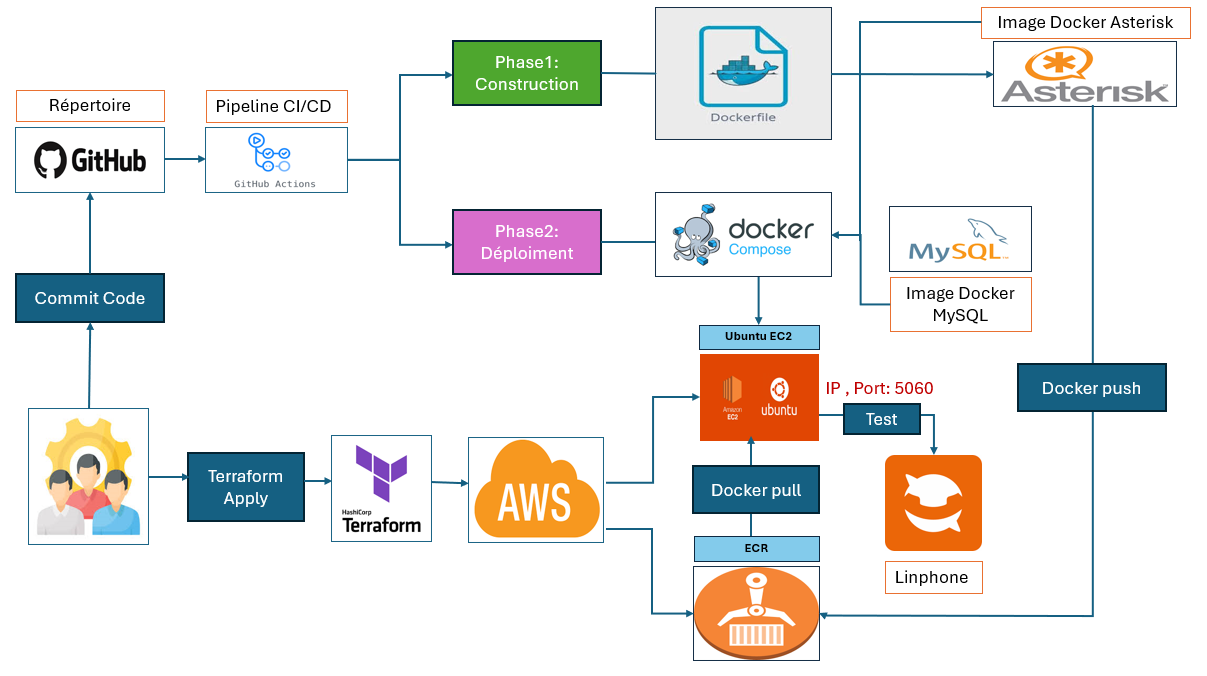
\includegraphics[width=17cm, height=12cm]{img/archi1.PNG}}
        \caption{Architecture de la solution proposée.}
        \label{fig:archi}
\end{figure}
        
Le passage à cette solution permet à l'entreprise de mieux maîtriser ses coûts, d'adapter l'outil à ses besoins spécifiques, et d'automatiser efficacement l'intégration et le déploiement de notre système de communication.

\section[Méthodologie de travail]{Méthodologie de travail}
Parmi les indispensables phases d’un projet, la définition d'une méthodologie de travail.

\subsection{Gestion de projet}
Pour garantir le bon déroulement de notre projet, nous adoptons la méthode Scrum. En effet, Scrum présente un cadre adapté pour gérer notre travail de manière efficace. Cette Méthodologie favorise la simplicité, l'agilité et la collaboration. De plus, elle vise à fixer la liste des tâches à effectuer en estimant pour chacune d’elle la durée de sa réalisation. Cela garantit la livraison d'un produit de haute qualité.

\subsection{Backlog du produit}
Dans cette section, nous présentons le backlog du produit (Product Backlog) qui est un élément crucial dans Scrum. Il sert à définir, organiser et prioriser les tâches à développer comme illustré dans le tableau \ref{tab:product_backlog}.

\begin{table}[h!]
    \centering
    \caption{Backlog du produit.}
    \begin{tabular}{|>{\centering\arraybackslash}m{1cm}|>{\centering\arraybackslash}m{3.5cm}|>{\centering\arraybackslash}m{4.5cm}|>{\centering\arraybackslash}m{1.5cm}|>{\centering\arraybackslash}m{2cm}|>{\centering\arraybackslash}m{2cm}|}
        \hline
        \textbf{ID} & \textbf{User Story} & \textbf{Description} & \textbf{Priorité} & \textbf{Difficulté} & \textbf{Durée} \\
        \hline
        1 & Étude comparative des outils DevOps & Réaliser une étude comparative des outils disponibles sur le marché afin d'identifier l'outil adapté & 3 & Moyenne & 2 semaines \\
        \hline
        2 & Implémentation d'une infrastructure & Implémenter une infrastructure cloud automatisée pour le déploiement de notre solution & 2 & Haute & 5 semaines \\
        \hline
        3 & Mise en place d'un pipeline CI/CD & Mettre en place une approche d'intégration et de déploiement continus en fonction des outils DevOps sélectionnés lors de l'étude comparative & 1 & Haute & 6 semaines \\
        \hline
        4 & Mise en place d'une configuration client-serveur & Mettre en place la configuration nécessaire pour établir une connexion client-serveur & 4 & Haute & 3 semaines \\
        \hline
    \end{tabular}
    \label{tab:product_backlog}
\end{table}

\section*{Conclusion}
Dans ce chapitre, nous avons traité le cadre général du projet, analysé la situation actuelle et la problématique, proposé une solution adéquate, et défini la méthodologie adoptée pour la réalisation de notre projet. Le chapitre suivant présentera un état de l'art sur les concepts fondamentaux de DevOps et du Cloud Computing. Nous y inclurons également une étude comparative des outils et technologies qui seront utilisés pour mettre en œuvre la solution.
% \chapter{Cadre et Contexte du travail}
% \section*{Introduction}
% Ce premier chapitre a pour objectif de contextualiser le projet dans son ensemble. Nous débutons par une présentation de l'organisme d'accueil. Ensuite, nous analysons la problématique actuelle en mettant en avant les limites et les difficultés rencontrées. Par la suite, nous proposons une solution adéquate. Enfin, nous concluons par une présentation de la méthodologie employée dans notre travail.
% % Une section
% \section{Organisme d'accueil}
% Cette section est consacré pour la description de l’organisme d’accueil lors de notre stage PFE, nous présentons également les services qu’il propose à ses clients. 

% \subsection{Présentation Générale}
% Notre projet de fin d’études est mené au sein de Luceor Labs, un fournisseur de réseaux IP sans file. L'entreprise a été fondée en 2005 et rachetée par le groupe Novatel en 2021, ce qui lui a permis de se doter d'un cadre technologique plus solide et plus innovant. C'est une société mondiale dont le siège se trouve à Paris et qui est présente en Europe, au Moyen-Orient et en Afrique.

% \subsection{Services et clients cibles}
%  Luceor Labs fournit des équipements de réseau sans fil, des packs de gestion logicielle et des solutions avancées de bout en bout. 
% Pour les organisations ayant des besoins de connectivité spécialisés, les produits Luceor simplifient la prise de décision et permettent la meilleure combinaison de couverture, de bande passante, de confidentialité et de sécurité. En outre, l'entreprise s'engage à fournir des solutions de communication de pointe aux clients qui opèrent dans des environnements exigeants où la sécurité et la fiabilité sont primordiales. Elle accompagne un large éventail de clients. Ces clients sont :

% \begin{itemize}
%     \item Les opérateurs d'entrepôts industriels et d'usines de marchandises ou de conteneurs
%     \item Les institutions de sécurité publique
%     \item Les responsables de la sécurité des événements
%     \item Les sociétés minières
%     \item Les Compagnies pétrolières et gazières
% \end{itemize}

% \section{Problématique}
% La mise en œuvre de tout projet doit être précédée d'une analyse approfondie de la problématique, soulignant les points faibles du système actuel et les difficultés rencontrées. Actuellement, Luceor utilise l'application "StreamWide Team On Mission" pour les communications lors des missions internes et des opérations critiques, ce qui facilite la coordination des tâches entre les membres de l'équipe. Cet outil nous offre une solution complète de gestion de communication, avec un accent particulier sur les fonctionnalités spécifiques aux missions critiques et sur la sécurité des données. Cependant, son coût élevé pousse l'entreprise à envisager le développement d'une solution interne plus abordable, basée sur le serveur Asterisk. La société souhaite disposer des fonctionnalités minimales d'un service de communications critiques, telles que les appels audio et vidéo, ainsi que l'intégration avec sa propre base de données. Lors de la phase de développement, le manque d'un mécanisme automatisé pour gérer les versions exécutables du code peut causer des problèmes de gestion et ralentir la mise en production du produit. De plus, l'absence d'automatisation dans l'approvisionnement de l'infrastructure oblige les développeurs à créer manuellement les ressources du serveur, ce qui est plus chronophage comparé à l'utilisation d'un script déployable en une simple commande. L'absence de ce processus nous empêche de redémarrer rapidement l'environnement en cas de défaillance. Finalement, la connexion au serveur nécessite une application cliente SIP open-source.

% \section[Solution proposée]{Solution proposée}
% Pour résoudre le problème mentionné précédemment, nous allons implémenter un serveur Asterik. Ce serveur doit être déployé automatiquement sur une infrastructure cloud public comme AWS. L'objectif de l'utilisation du cloud est de rendre le serveur accessible à l'équipe de développement, libérant ainsi les développeurs des contraintes du travail en local et facilitant la communication des clients distants à travers différents réseaux.
% De plus, l'utilisation d'une infrastructure en tant que code (IaC) nous permet d'allouer des ressources AWS comme une instance ubuntu EC2 et un dépot ECR de stockage des conteneurs. L'automatisation de création de notre propre infrastructure s'appuie sur Terraform comme outil d'IaC.  Après l'approvisionnement de l'infrastructure, notre solution doit inclure un pipeline CI/CD à travers GitHub Actions pour gérer la construction de notre serveur Asterisk et automatiser son déploiement dans l'instance EC2 comme étant un environnement de pré-production. Ce pipeline se déclenche à chaque fois que du code est livré sur l'outil de gestion des versions GitHub, dès qu'il y a des modifications. Cela assure une synchronisation efficace des codes sources et renforce la continuité offerte par l'approche DevOps. Le pipeline comprend deux phases. La première consiste à développer un processus de création d'une version exécutable pour Asterisk moyannant Dockerfile. Ensuite, nous stockons cette image dans le service de stockage des conteneurs ECR d’ AWS. La deuxième phase concerne le déploiement du serveur sur le cloud en utilisant l'image Docker stockée dans notre répertoire ECR. Durant cette phase, nous devons également lancer le service Asterisk avec un serveur base de données MySQL en utilisant Docker-Compose.
% Une fois le pipeline est terminé avec succès, nous pouvons tester et effectuer des appels avec une application client SIP open-source. Linphone s'avère être la meilleure option, et nous envisageons de la personnaliser par la suite.
% La figure \ref{fig:archi} illustre l'architecture de notre solution dont nous avons mentionné tous les outils et technologies nécessaire pour sa mise en place.
% \begin{figure}[H]
%         \centering
%        \frame{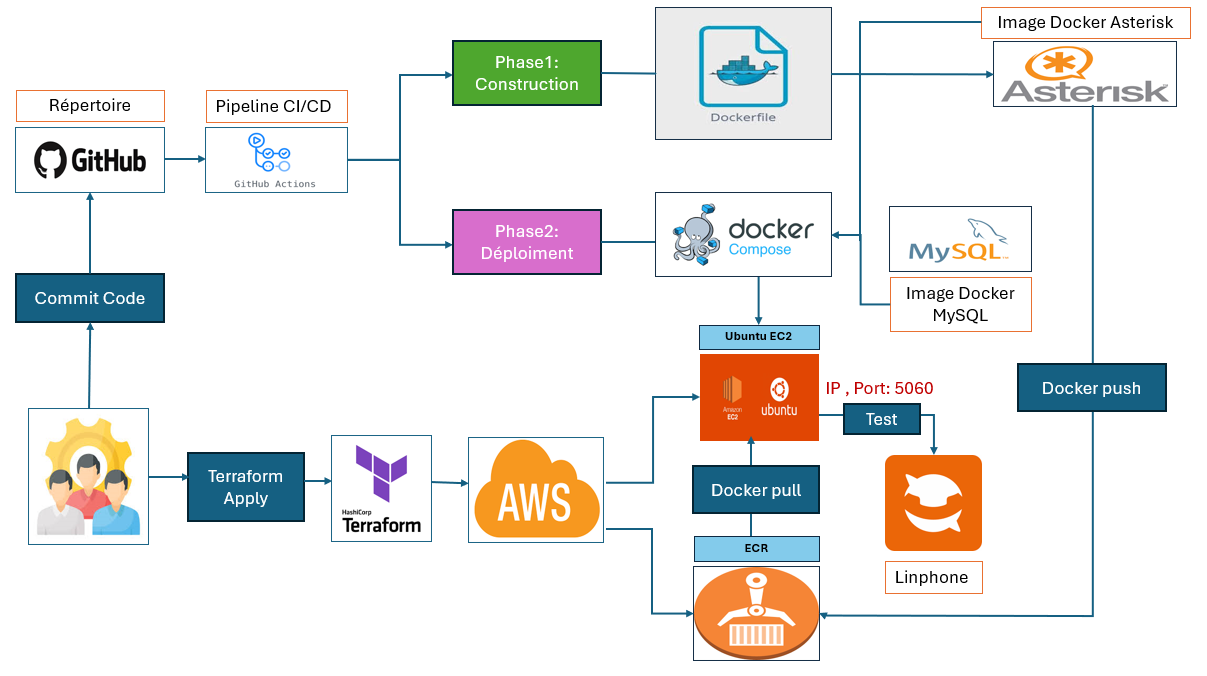
\includegraphics[width=17cm, height=10cm]{img/archi1.PNG}}
%         \caption{Architecture de la solution proposée.}
%         \label{fig:archi}
% \end{figure}
        
% Le passage à cette solution permet à l'entreprise de mieux maîtriser ses coûts, d'adapter l'outil à ses besoins spécifiques, et d'automatiser efficacement l'intégration et le déploiement de notre système de communication.

% \section[Méthodologie de travail]{Méthodologie de travail}
% \subsection{Gestion de projet}
% Pour garantir le bon déroulement de notre projet, nous adoptons la méthode Scrum. En effet, Scrum présente un cadre adapté pour gérer notre travail de manière efficace. Cette Méthodologie favorise la simplicité, l'agilité et la collaboration. De plus, elle vise à fixer la liste des tâches à effectuer en estimant pour chacune d’elle la durée de sa réalisation. Cela garantit la livraison d'un produit de haute qualité.
% \begin{table}
%     \centering
%     \caption{Backlog du produit.}
%     \begin{tabular}{|>{\centering\arraybackslash}m{1cm}|>{\centering\arraybackslash}m{3cm}|>{\centering\arraybackslash}m{5cm}|>{\centering\arraybackslash}m{1.5cm}|>{\centering\arraybackslash}m{2cm}|>{\centering\arraybackslash}m{2cm}|}
%         \hline
%         \textbf{ID} & \textbf{User Story} & \textbf{Description} & \textbf{Priorité} & \textbf{Difficulté} & \textbf{Durée} \\
%         \hline
%         1 & Étude comparative des outils DevOps & Réaliser une étude comparative des outils disponibles sur le marché afin d'identifier l'outil adapté & 3 & Moyenne & 2 semaines \\
%         \hline
%         2 & Implémentation d'une infrastructure & Implémenter une infrastructure cloud automatisée pour le déploiement de notre solution & 2 & Haute & 5 semaines \\
%         \hline
%         3 & Mise en place d'un pipeline CI/CD & Mettre en place une approche d'intégration et de déploiement continus en fonction des outils DevOps sélectionnés lors de l'étude comparative & 1 & Haute & 6 semaines \\
%         \hline
%         4 & Mise en place d'une configuration client-serveur & Mettre en place la configuration nécessaire pour établir une connexion client-serveur & 4 & Haute & 3 semaines \\
%         \hline
%     \end{tabular}
%     \label{tab:product_backlog}
% \end{table}

% \subsection{Backlog du produit}
% Dans cette section, nous présentons le backlog du produit (Product Backlog) qui est un élément crucial dans Scrum. Il sert à définir, organiser et prioriser les tâches à développer comme illustré dans le tableau \ref{tab:product_backlog}.



% \section*{Conclusion}
% Dans ce chapitre, nous avons traité le cadre général du projet, analysé la situation actuelle et la problématique, proposé une solution adéquate, et défini la méthodologie adoptée pour la réalisation de notre projet. Le chapitre suivant présentera un état de l'art sur les concepts fondamentaux de DevOps et du Cloud Computing. Nous y inclurons également une étude comparative des outils et technologies qui seront utilisés pour mettre en œuvre la solution.

        \clearpage
        
        \chapter{Etat de l'art}
\section*{Introduction}
Dans ce chapitre, Nous analysons les principales pratiques et les outils les plus adaptés à notre projet. Nous commençons par introduire les concepts de DevOps, CI/CD, Cloud Computing et IaC. Après, nous mettons l'accent sur l’intégration du cloud dans notre solution DevOps et l'intégration de l'IaC dans notre solution cloud. En conclusion, nous effectuons une analyse comparative des outils tout en synthétisant nos choix optés.

\section{Approche DevOps}
L'approche DevOps \cite{crochetdamais2019} regroupe un ensemble de techniques qui met en relief l'automatisation des tâches entre l'équipe de développement de logiciels (Dev) et l'équipe d'exploitation informatique (Ops), comme le montre la figure \ref{fig:devops} \cite{kim2022}.
        \begin{figure}[H]
        \centering
        \frame{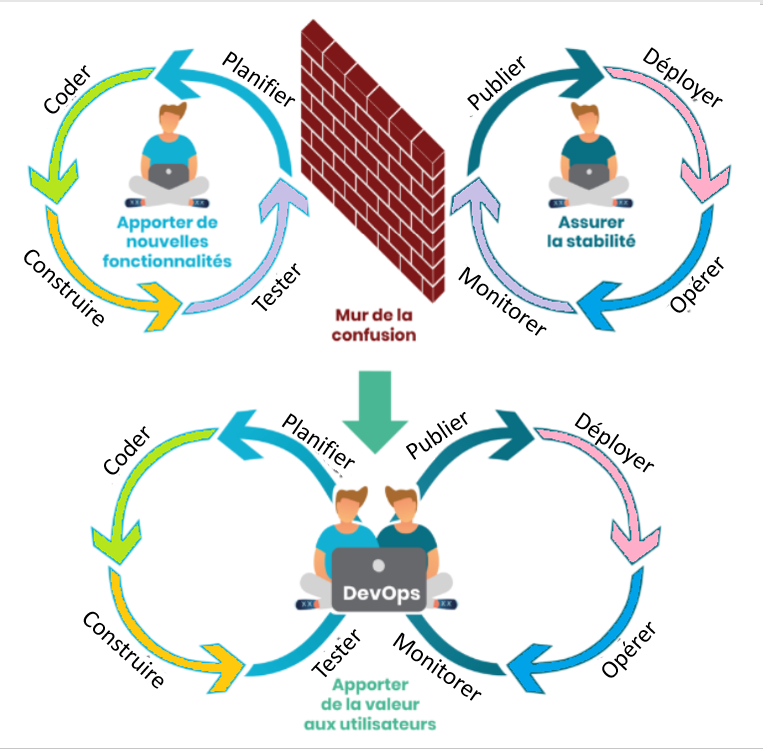
\includegraphics[width=16cm, height=12cm]{img/5.png}}
        \caption{Approche DevOps.}
        \label{fig:devops}
        \end{figure}
Les deux équipes alors se collaborent ensemble du début à la fin du cycle de vie des applications, depuis le développement et les tests, jusqu' au déploiement et à l'exploitation. Le but est d'accélérer la livraison des applications par rapport aux méthodes de développement traditionnelles. Cette collaboration améliore la réactivité de l'entreprise, la rendant plus compétitive et plus apte à satisfaire ses clients sur le marché.

\section{Intégration continue et déploiement continu CI/CD}

Le CI/CD est une technique clé dans l'approche DevOps, composée de deux pratiques fondamentales : l'intégration continue (CI) et la livraison et déploiement continus (CD).\\
L'intégration continue (CI) \cite{moronval2020} permet de fusionner fréquemment les modifications de code et déclenche un processus automatisé de construction et de test pour vérifier le bon fonctionnement de l'application. Cette pratique vise à identifier rapidement les conflits ou les erreurs dans le code, permettant ainsi de les résoudre de manière efficace et rapide. En cas de conflit entre le code actuel et le nouveau code ou en cas d'erreur dans le code, la CI intervient immédiatement pour résoudre le problème, minimisant ainsi les interruptions de développement. \\
La livraison continue va un pas plus loin en s'assurant que le code validé est toujours dans un état déployable. Alors que, Le déploiement continu (CD) \cite{crochetdamais2023}, complète l'intégration et la livraison continues. Il garantit que les modifications validées sont automatiquement déployées dans un environnement de production, tel que le cloud. Cette pratique permet de minimiser les risques associés aux déploiements manuels et de rendre les nouvelles fonctionnalités immédiatement disponibles aux utilisateurs.\\
Le déploiement continu assure une livraison fluide et ininterrompue des mises à jour, facilitant une réponse rapide aux retours des utilisateurs et aux besoins du marché. La figure \ref{fig:cid} \cite{veritis2024} indique les éléments de pipeline les plus courantes.
        \begin{figure}[H]
        \centering
        \frame{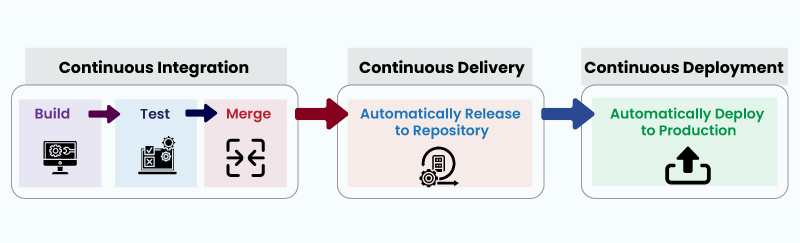
\includegraphics[width=16cm, height=6.5cm]{img/continuous-deployment.jpg}}
        \caption{Éléments de pipeline CI/CD.}
        \label{fig:cid}
        \end{figure}

\section{Conteneurisation et virtualisation cloud}
La virtualisation et la conteneurisation sont deux technologies utilisées lors de la phase de déploiement. Nous allons maintenant les introduire. La conteneurisation \cite{axopen2021docker} repose sur l'utilisation de logiciels tels que Docker, permettant de se passer d'un système d'exploitation distinct pour chaque conteneur. Ce concept est illustré par la figure \ref{fig:cont} \cite{strauss2020}. Dans ce contexte, toutes les dépendances de l'application sont regroupées dans un conteneur. Les ressources, telles que l'espace et la mémoire, ne sont pas fixées, mais allouées en fonction des besoins de l'application, éliminant ainsi la surcharge. Cette approche offre de meilleures performances en termes de rapidité et de légèreté. Nous l'utiliserons ensuite pour créer nos conteneurs Asterisk et MySQL.
\begin{figure}[H]
        \centering
        \frame{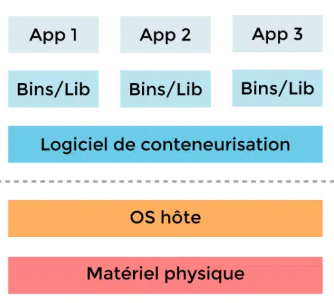
\includegraphics[width=7.5cm, height=5cm]{img/Conteneurisation.PNG}}
        \caption{Conteneurisation.}
        \label{fig:cont}
        \end{figure}
Cependant, la virtualisation \cite{samarakoon2023} repose sur un hyperviseur pour créer et exécuter plusieurs machines virtuelles sur un système hôte, comme le montre la figure \ref{fig:virtual} \cite{strauss2020}. Chaque machine virtuelle possède son propre système d'exploitation. 
\begin{figure}[H]
        \centering
        \frame{\includegraphics[width=7.5cm, height=6.5cm]{img/virtual.PNG}}
        \caption{Virtualisation.}
        \label{fig:virtual}
        \end{figure}
Cette approche peut surcharger la plate-forme hôte puisque des quantités fixes de mémoire et d'espace sont allouées à chaque machine virtuelle, ce qui peut entraîner un gaspillage significatif de ressources. D'où, nous décisions de passer à La virtualisation cloud qui présente plusieurs avantages significatifs en termes de flexibilité et de gestion des ressources. Les fournisseurs de Cloud Computing utilisent cette technologie pour optimiser l'utilisation des ressources physiques, créant ainsi des environnements isolés et sécurisés pour chaque utilisateur. Cela permet de provisionner, déployer et gérer facilement nos ressources tout en répondant aux besoins de l'entreprise et en maximisant l'efficacité opérationnelle.

\section{Cloud Computing}
Le Cloud Computing \cite{Plu2019} ou l'informatique en nuage présente un service qui fournit un ensemble de ressources informatiques accessibles via Internet. Il offre la possibilité de stocker et de gérer les données, les logiciels et les applications sur des serveurs. Nous pouvons le classer en trois types, selon le mode d'hébergement, comme indiqué dans la figure \ref{fig:cloud} \cite{syloe2018}.
        \begin{figure}[H]
        \centering
        \frame{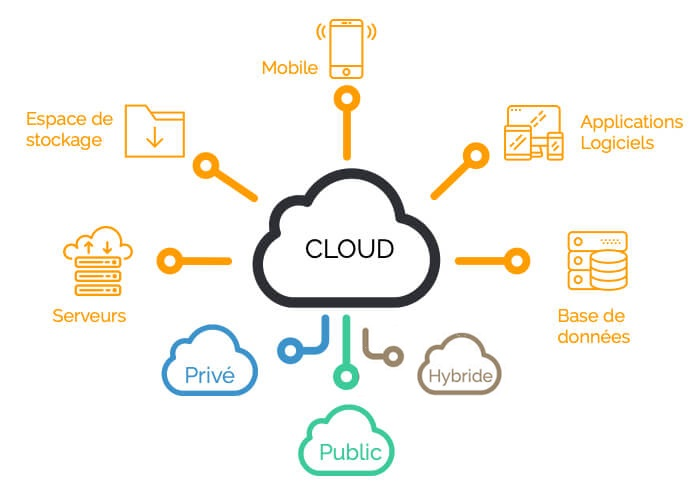
\includegraphics[width=16cm, height=9cm]{img/schema-cloud.jpg}}
        \caption{Types de Cloud Computing.}
        \label{fig:cloud}
        \end{figure}
\begin{itemize}
    \item \textbf{Cloud public} : il met à disposition des ressources publiques fournies par un fournisseur tiers. Il permet à de multiples utilisateurs d'accéder aux mêmes services et infrastructures via Internet. C'est une solution économique et évolutive, idéale pour les applications non sensibles aux données et nécessitant une évolutivité rapide.
    \item \textbf{Cloud privé} : il propose des services cloud propres à une entreprise, accessibles uniquement en interne, afin de garder la main sur l'infrastructure et répondre aux exigences strictes en matière de sécurité et de conformité.
    \item \textbf{Cloud hybride} : il s'agit d'une combinaison du cloud public et du cloud privé, où l'entreprise utilise ses propres ressources internes pour des tâches critiques tout en exploitant des ressources cloud publiques pour des opérations moins sensibles aux données. Cela offre une plus grande flexibilité et optimise les coûts en fonction des besoins spécifiques de l'organisation.
\end{itemize}
\section{Approche IaC}
L’infrastructure as code (IaC) sert à écrire un code qui automatise la création et la configuration de l'infrastructure informatique à travers des langages de codage descriptifs de haut niveau. Grâce à cette automatisation, l'équipe DevOps n’a plus besoin de configurer et de gérer manuellement les ressources chaque fois qu’ils développent, testent ou déploient une application logicielle.
Grâce à l'IaC, les environnements d'infrastructure, tels que les serveurs, les réseaux et les bases de données, peuvent être définis et gérés de manière cohérente et reproductible. Cela simplifie le processus de déploiement et garantit que l'infrastructure est toujours configurée de manière optimale et conforme aux besoins de l'application. Par exemple, en utilisant des outils comme Terraform, les équipes peuvent décrire leur infrastructure cible dans des fichiers de configuration. Ces fichiers sont ensuite exécutés pour déployer et mettre à jour automatiquement les ressources nécessaires, que ce soit dans des environnements locaux, dans le cloud ou dans des architectures hybrides. Cela permet de réduire les erreurs humaines, d'améliorer la sécurité et de simplifier la gestion globale des infrastructures informatiques.

\section{Intégration de Cloud Computing dans la solution DevOps}
L’objectif d’une solution DevOps est d’accélérer la mise en production des applications tout en présentant une meilleure qualité. Bien que DevOps soit une approche indépendante du cloud, ce dernier joue un rôle très important pour renforcer son efficacité. Il sert à simplifier la mise en place et la gestion de l’infrastructure nécessaire pour l’exécution d’une application. Grâce au cloud, les équipes DevOps peuvent facilement provisionner et configurer des environnements d'exécution, ce qui permet une intégration continue rapide et une livraison continue des applications. Cela conduit à une satisfaction accrue de l'utilisateur final, car les mises à jour et les nouvelles fonctionnalités sont déployées plus rapidement et de manière plus fiable. De plus, le cloud offre une solution économique pour le déploiement des applications, car il permet de réduire les coûts liés à l'achat et à la gestion d'infrastructures physiques. Les fournisseurs de cloud proposent également une gamme étendue d'outils et de services qui simplifient les opérations de développement et d'exploitation, comme le stockage de données, la gestion des identités, et les services de sécurité.

\section{Intégration de l'approche IaC dans le Cloud Computing}
Le cloud computing favorise l'approche Infrastructure as Code (IaC). Grâce à cette méthode, nous pouvons créer, modifier et supprimer nos ressources cloud en utilisant un code automatisé. Cela contribue à la rapidité et à la facilité de gestion de l'infrastructure cloud. En utilisant des outils comme Terraform, Ansible, ou CloudFormation, les équipes peuvent décrire leur infrastructure cible dans des fichiers de configuration. Ces fichiers sont ensuite exécutés pour déployer et mettre à jour automatiquement les ressources nécessaires dans le cloud. Cette automatisation permet de réduire les erreurs manuelles, d'améliorer la cohérence et de garantir que l'infrastructure est toujours configurée de manière optimale. De plus, l'IaC facilite la reproductibilité et la scalabilité des environnements cloud. Les configurations peuvent être répliquées facilement d'un environnement à un autre, par exemple, du développement à la production, assurant ainsi une uniformité et une conformité constantes.

\section{Etude comparative des outils}
Il existe différents outils sur le marché pour notre solution proposée, ce qui rend le choix difficile, d'où la nécessité d'une étude comparative pour faire le bon choix selon nos besoins.

\subsection{Outils de gestion des versions}
La gestion des versions \cite{axopen} enregistre les changements apportées au code source d'une application, facilitant la collaboration entre l'équipe et la récupération de versions spécifiques. Elle permet le travail sur plusieurs branches, la gestion des modifications, et la résolution des problèmes de fusion.
Cette étude sur la gestion des versions, illustrée dans le tableau \ref{tableau:comparatif3} \cite{strauss2018}, vise à consolider le choix de l'outil GitHub, déjà utilisé en interne, par rapport à ses concurrents GitLab et BitBucket.
\begin{table}[H]
\centering
\caption{Tableau comparatif des outils de gestion des versions GitHub, Gitlab et Bitbucket.}
\begin{longtable}{|p{3.5cm}|p{3.75cm}|p{3.75cm}|p{3.75cm}|}
\hline
\textbf{Critères de comparaison} & \textbf{GitHub Entreprise} & \textbf{GitLab Ultimate} & \textbf{Bitbucket Premium}\\
\hline
\textbf{Propriétaire} & Microsoft & GitLab Inc. & Atlassian \\
\hline
\textbf{Language} & Ruby & Ruby, Go, Vue.js & Python\\
\hline
\textbf{Open-source} & Non & Oui & Non \\
\hline
\textbf{Integrations} & Jira, Microsoft Teams, Slack, Microsoft Azure & Jira, Bugzilla, Custom Issue, Tracker & Jira, Trello, Bamboo, Opsgenie \\ 
\hline
\textbf{CI/CD en minutes par mois} &  50.000 &  50.000 & 3.500 \\
\hline
\textbf{Limite de stockage} & 50 GB  &  60\$ pour chaque ajout de 10 GB & 10 GB \\
\hline
\textbf{Coût d'un utilisateur par mois} & 21\$ & 99\$ & 6\$\\
\hline
\textbf{Communauté} & Robuste & Active & Limitée\\
\hline
\end{longtable}
\label{tableau:comparatif3}
\end{table}
GitHub est l'outil choisi, étant donné qu'il propose diverses fonctionnalités de gestion des versions. Il offre une grande variété d'intégrations avec des outils couramment utilisés. De plus, GitHub Actions fournit un temps d'exécution important pour les pipelines CI/CD, et des limites de stockage largement flexibles pour répondre à nos besoins. Il dispose également d'une communauté solide. En outre, il présente l'avantage d'être moins coûteux que GitLab et GitLab CI/CD.

\subsection{Outils de conteneurisation}
Docker et Podman sont les plus populaires outils de conteneurisation. Le tableau \ref{tableau:comparatif2} \cite{aleksic2022} permet de comparer ces deux outils afin de retenir l’outil qui satisfait au mieux les besoins de l’entreprise.
\begin{table}[H]
\centering
\caption{Tableau comparatif des outis de conteneurisation Docker et Podman.}
\begin{longtable}{|p{4.5cm}|p{5.5cm}|p{5.5cm}|}
\hline
\textbf{Critères de comparaison} & \textbf{Docker} & \textbf{Podman} \\
\hline
\textbf{Technologie de conteneur} & Utilise Docker Engine & Utilise le moteur Podman \\
\hline
\textbf{Architecture} & Utilise le démon Docker & Sans démon \\
\hline
\textbf{Privilèges de l'utilisateur} & Super utilisateur & Super utilisateur et utilisateur ordinaire \\
\hline
\textbf{Images} & Création d'images de conteneur & Utilise Buildah pour créer des images de conteneur \\ 
\hline
\textbf{Orchestration} & Docker Swarm, utilisable avec Kubernetes & Utilisable avec Kubernetes  \\ 
\hline
\textbf{Utilisation dans l'industrie} & Largement utilisé et bien documenté & Outil plus récent, moins utilisé, documentation moins abondante\\
\hline
\textbf{Système d'exploitation} & Linux, Windows, macOS & Linux, Windows (avec WSL), macOS\\
\hline
\end{longtable}
\label{tableau:comparatif2}
\end{table}

Après une analyse comparative, notre choix s'est porté sur Docker en raison de sa large adoption, de ses performances fiables grâce à Docker Engine, et de sa flexibilité. Il repose sur une architecture client-serveur avec un démon. Il bénéficie d'une documentation complète. De plus, cet outil propose Docker Swarm pour l'orchestration des conteneurs, et peut également être intégré avec Kubernetes. Le logiciel est aussi compatible avec plusieurs systèmes d'exploitation, présentant alors un choix solide pour notre équipe DevOps.

\subsection{Outils d'approvisionnement de l'infrastructure}
Grâce à des outils d'approvisionnement de l'infrastructure, nous n'avons pas besoin de créer nos ressources manuellement, il suffit d'exécuter le code de notre infrastructure qui effectue toute la configuration sur le cloud.
Le tableau \ref{tableau:terraform} \cite{Kadima2024} synthétise une série de critères de comparaison entre Terraform et Ansible permettant de trancher sur l’outil IaC qui satisfait au mieux les besoins de l’entreprise.
\begin{table}[H]
\centering
\caption{Tableau comparatif des outils de gestion et d’automatisation des configurations Terraform et Ansible.}
\begin{longtable}{|p{4.5cm}|p{5.25cm}|p{5.25cm}|}
\hline
\textbf{Critères de comparaison} & \textbf{Terraform} &\textbf{Ansible} \\ 
\hline
\textbf{Type} & Infrastructure as Code (IaC) & Configuration Management \\
\hline
\textbf{Architecture} & Sans agent & Sans agent \\
\hline
\textbf{Language} & HCL & YAML/Ansible Playbooks\\
\hline
\textbf{Syntaxe} & Déclarative & Impérative \\
\hline
\textbf{Installation} & Facile & Facile \\
\hline
\textbf{Support des clouds} & Multi-cloud & Multi-cloud \\
\hline
\textbf{Approche par défaut} & Approvisionnement et orchestration des infrastructures & Configuration et gestion des états des systèmes \\
\hline
\textbf{Gestion du cycle de vie des ressources} & Complet (création, mise à jour, destruction) & Partiel (principalement configuration et orchestration) \\
\hline
\textbf{Evolutivité} & Très rapide & Très rapide \\
\hline
\textbf{Communauté} & Grande et en croissance & Très grande \\
\hline
\end{longtable}
\label{tableau:terraform}
\end{table}
Nous avons choisi Terraform pour son expertise en approvisionnement et gestion d'infrastructure multi-cloud, ainsi que pour sa capacité à automatiser la gestion des ressources cloud avec une architecture sans agent. Sa communauté en croissance et son utilisation d'un langage dédié (HCL) en font un outil puissant et convivial pour la gestion d'infrastructure.

\subsection{Solution cloud public}
Le choix entre les trois types de cloud présentés dans la section 2.4 diffère d'une entreprise à une autre selon ses besoins. Luceor Labs a opté l'implémentation de son infrastructure sur un cloud public pour plusieurs avantages \cite{Ranger2022} :
\begin{itemize}
\item  \textbf{Coût}: le cloud public présente un faible coût et une tarification à l'usage, c'est-à-dire, nous ne payons que pour les ressources que nous consommons.
 \item  \textbf{Accessibilité}: ce cloud est accessible à tous grâce à Internet, ce qui simplifie la collaboration et l'accès aux données et aux applications.
\item  \textbf{Évolutivité}: les moyens évolutifs du cloud public permettent d'ajuster les ressources selon les besoins de l'entreprise.
\item  \textbf{Diversité}: une large gamme de services est offerte par le cloud public pour répondre aux demandes actuelles des entreprises.
% \item  \textbf{Flexibilité}: les solutions cloud sont flexibles, ce qui permet de personnaliser l'infrastructure d'une entreprise.
\item  \textbf{Maintenance}: la maintenance matérielle et logicielle est gérée par les fournisseurs, ce qui nous décharge de ces tâches techniques.
\item  \textbf{Sécurité}: les fournisseurs de cloud public offrent des solutions hautement sécurisées pour protéger les données des entreprises.
% \item  \textbf{Rapidité}: Il offre la rapidité de déploiement des applications. 

\end{itemize}
Amazon Web Services, Microsoft Azure ainsi que Google Cloud Platform sont les trois géants du cloud public qui dominent le marché, de sorte que le choix entre les trois options doit se fonder sur des critères très précis. Le tableau \ref{tableau:comparatif7} \cite{gil2023} présente une étude comparative de ces trois solutions.
\begin{table}[H]
\centering
\caption{Tableau comparatif des solutions cloud public AWS, Microsoft Azure et Google Cloud.}
\begin{longtable}{|p{3cm}|p{4cm}|p{4cm}|p{4cm}|}
\hline
\textbf{Critères de comparaison} & \textbf{AWS} & \textbf{Microsoft Azure} & \textbf{Google Cloud}\\
\hline
\textbf{Place sur le marché} & Leader mondial & Deuxième mondiale & Troisième mondiale \\
\hline
\textbf{Étendue géographique} & 102 zones de disponibilité réparties dans 32 régions & Plus de 60 régions & 39 régions \\
\hline
\textbf{Nombre de services} & Plus de 200 services & Plus de 200 services et intégration avec les produits Microsoft & Plus de 100 services\\
\hline
\textbf{Principaux utilisateurs} &  Netflix, Nasa, Samsung &  Boeing, eBay, Coca-Cola & Spotify, Twitter, PayPal \\
\hline
\textbf{Coût et tarification} & Tarification diversifiée avec une grande flexibilité  & Tarification flexible avec des réductions pour les clients existants & Offre compétitive avec des réductions pour l'utilisation continue \\ 
\hline
\end{longtable}
\label{tableau:comparatif7}
\end{table}
Nous avons choisi AWS comme cloud public pour plusieurs raisons. Tout d'abord, AWS occupe la première place mondiale parmi ses concurrents de services cloud, confirmant ainsi sa forte présence sur le marché. Ensuite, cette solution cloud offre une couverture géographique étendue, garantissant une disponibilité continue des services. En outre, elle fournit une série de services adaptés à nos besoins. Ses grands utilisateurs, tels que Netflix, la Nasa et Samsung, démontrent l'excellence des services qu'elle propose. Enfin, la tarification flexible d'AWS nous permet de contrôler efficacement nos coûts.
% %%%%%%%%%%%%%%%%%%%%%%%%%%%%%%%%%%%%%%%%%%%%%%%%%%%%%%%

\section{Synthèse et choix}
Suite à l'étude comparative des outils DevOps et à l'étude comparative d'une solution cloud public, présentées dans les deux sections précédentes, nous avons choisi plusieurs outils parfaitement adaptés à nos besoins. Nos choix technologiques sont présentés dans le tableau \ref{tableau:choix}.

\begin{table}[H]
\centering
\caption{Tableau récapitulatif des choix technologiques.}
\begin{longtable}{|p{10cm}|p{4cm}|}
\hline
\textbf{Catégorie} & \textbf{Outil} \\
\hline
Outils de gestion de version & GitHub  \\
\hline
Outils de conteneurisation & Docker \\
\hline
Outils d'approvisionnement de l'infrastructure  & Terraform \\
\hline
Solutions cloud public & AWS \\
\hline
\end{longtable}
\label{tableau:choix}
\end{table}

\section*{Conclusion}
A travers ce chapitre, nous avons exposé les concepts de base qui nous permettent de comprendre et de mener à bien notre projet, ainsi que les outils et les technologies choisis pour mettre en place notre solution. Dans le chapitre suivant, nous présenterons en détail l’analyse des besoins et l’environnement logiciel du travail

        \clearpage
        
        \chapter{Analyse des besoins et conception}
\section*{Introduction}
Ce chapitre a pour objectif de planifier la réalisation du projet. Nous commençons par analyser les différents besoins ainsi que l'architecture technique de notre projet. Nous terminons par une description des divers outils que nous avons utilisés tout au long du processus de mise en œuvre de notre solution.
\section{Spécification des besoins}
Dans cette partie, nous nous concentrons sur la spécification des besoins pour guider la création du projet et déterminer les attentes de l'entreprise afin de clarifier les objectifs. Nous distinguons deux types de besoins, es besoins fonctionnels qui expriment les tâches que le système doit effectuer en réponse à une demande et les besoins non fonctionnels qui expriment les exigences implicites que le système doit avoir.

\subsection{Besoins fonctionnels}
Les besoins fonctionnels se diffèrent selon les exigences spécifiques d’une entreprise ou d’un projet. nous décrivons alors les besoins fonctionnels requis pour notre solution :
\begin{itemize}
    \item \textbf{Passage des appels via Asterisk} :
    Permettre la réalisation d'appels entre les membres de l'équipe via le serveur Asterisk à implémenter, en garantissant une qualité de service optimale pour les communications critiques.

    \item \textbf{Intégration avec la base de données interne} :
    Intégrer le serveur Asterisk avec une base de données MySQL propre à l'entreprise pour stocker les informations des utilisateurs, facilitant ainsi la gestion et l'analyse des données.

    \item \textbf{Automatisation de l'approvisionnement} :
    Utiliser Terraform comme outil d'infrastructure en tant que code (IaC) pour automatiser l'allocation des ressources nécessaires sur le cloud AWS, incluant les instances EC2 et le service de stockage de conteneurs ECR.

    \item \textbf{Dockerisation des serveurs Asterisk et MySQL} :
    Construire et conteneriser les images Docker pour les serveurs Asterisk et MySQL, assurant ainsi une portabilité et une facilité de déploiement dans différents environnements.

    \item \textbf{Stockage des images Docker} :
    Stocker les images Docker dans un service de stockage sur un cloud public, tel que le registre de conteneurs ECR d'AWS, pour une gestion centralisée et sécurisée des images.

    \item \textbf{Gestion de versions du code} :
    Gérer les branches et les versions du code source en utilisant Git, facilitant ainsi la collaboration entre les développeurs et le suivi des modifications du code.

    \item \textbf{Intégration continue} :
    Implémenter un pipeline CI avec GitHub Actions pour automatiser la construction des images Docker à chaque modification du code source, garantissant ainsi une livraison continue des nouvelles fonctionnalités et correctifs.

    \item \textbf{Déploiement continu} :
    Utiliser GitHub Actions pour automatiser le déploiement continu du serveur Asterisk sur le cloud, en déployant les images Docker stockées dans ECR sur les instances EC2, assurant ainsi une mise à jour rapide et fiable de l'environnement de pré-production.

    \item \textbf{Application cliente SIP} :
    Configurer et personnaliser une application cliente SIP open-source, comme Linphone, pour permettre aux utilisateurs de se connecter au serveur Asterisk et de tester les fonctionnalités d'appel.

        \item \textbf{Sécurité} :
    Assurer la sécurité des données, en mettant en place des mesures de protection adéquates pour le serveur Asterisk et la base de données MySQL.
    
    \item \textbf{Disponibilité} :
    Garantir une haute disponibilité du serveur Asterisk pour les utilisateurs.
\end{itemize}

\subsection{Besoins non fonctionneles}
En plus des besoins fonctionnels, nous spécifions les besoins non fonctionnels requis pour notre solution :

\begin{itemize}


    \item \textbf{Évolutivité} :
    Permettre une montée en charge facile du système en cas d'augmentation du nombre d'utilisateurs ou du volume de communications, en utilisant des solutions cloud pour ajuster les ressources en fonction des besoins.

    \item \textbf{Coût} :
    Réduire les coûts de fonctionnement par rapport à l'utilisation de l'application "StreamWide Team On Mission", en utilisant des solutions open-source et cloud pour maîtriser les dépenses.

    \item \textbf{Maintenabilité} :
    Faciliter la maintenance et les mises à jour du système grâce à l'utilisation de conteneurs et d'un pipeline CI/CD, et assurer une documentation complète et claire du processus de déploiement et de gestion du serveur.
\end{itemize}

\section{Architecture technique du projet}
L’utilisation d’une infrastructure en tant que code (IaC) permet d’allouer des ressources sur AWS et d’automatiser la création de notre propre infrastructure de déploiement. Cette automatisation s’appuie sur Terraform, un outil d’IaC, pour provisionner et gérer les ressources nécessaires de manière efficace et reproductible.\\
Pour connecter à notre cloud public, Il nous faut un compte
IAM (Identity and Access Management). Suite à l’exécution du code via la commande Terraform Apply, les ressources cloud seront créées. Ces derniers sont un registre des conteneurs (ECR), un réseau virtuel privé (VPC) avec un subnet public et un internet getway, un groupe de sécurité qui définit les règles d’accès à notre instance ubuntu EC2, un table de routage et son association avec le subnet créé, un générateur de clé privée et un générateur de clé public. La clé privée générée au sein de l’instance EC2 doit être copiée dans la machine locale pour connecter à l’instance via SSH. Dès que notre instance est lancée, un script bash sera executé pour y installer Docker et Git.\\ D'autre part, GitHub Actions se charge de déclencher le pipeline CI/CD suite à la détection d'un changement du code sur le répertoire Git. Ce pipeline assure la construction de notre serveur Asterisk et automatise son déploiement sur l'instance ubuntu. \\Donc, il se compose de deux phases, la première phase sert à créer une image Docker d'Asterisk en utilisant un Dockerfile la stocker dans ECR via la commande Docker Push. La deuxième phase c'est le déploiement de l'application sur AWS. L'image Docker stockée dans ECR sera copiée en local via la commande Docker Pull et lancée avec un serveur de base de données MySQL sur l'instance cloud en utilisant Docker-Compose, favorisant que les deux services fonctionnent respectivement sur les ports 5060 et 3306.\\ Après le déploiement, nous pouvons tester et effectuer des appels avec Linphone en tapant le nom de domaine IP du serveur Asterisk, le nom d'utilisateur et le mot de passe. La figure \ref{fig:archi_glob} illustre l'architecture technique de notre solution.
\begin{figure}[H]
        \centering
       \frame{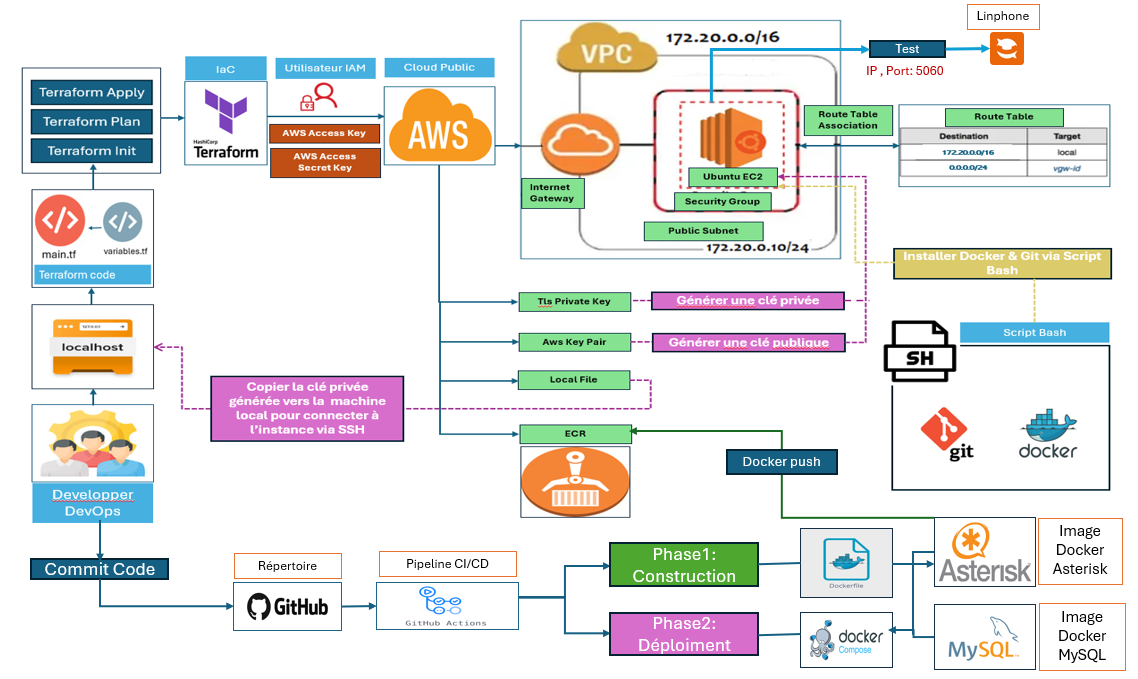
\includegraphics[width=17cm, height=14cm]{img/archi_détaillée.PNG}}
        \caption{Architecture technique du projet.}
        \label{fig:archi_glob}
\end{figure}

\section{Environnement de travail}
Durant cette partie, nous présentons les outils matériels et logiciels de notre projet. 

\subsection{Environnement de travail matériel}
L'ordinateur portable utilisé pour réaliser notre projet présente les caractéristiques suivantes :
\begin{itemize}
\item {Système d’exploitation : Windows 11 Pro}
\item {Processeur :  Intel Core i7-8565U, 4.6 GHz} 
\item {Mémoire installé (RAM): 16 Go}
\item {Disque dur : 1 To}
\end{itemize}

\subsection{Environnement de travail logiciel}
Avant de passer à la réalisation, nous identifions les technologies utilisées durant ce projet.

\subsubsection{Jira Software}
Jira Software présente un moyen de planification et de suivi des tâches d'un projet, développé par Atlassian. Il simplifie la collaboration et favorise l'agilité.

\subsubsection{Visual Studio Code}
Comme dans tout projet informatique, nous avons besoin d'un éditeur de code source comme Visual Studio Code. Ce logiciel développé par Microsoft est gratuit et open-source.

\subsubsection{Qt5}
Qt5 est un framework multiplateforme qui fournit des outils puissants pour la création d'interfaces utilisateur, la gestion des événements, et la communication inter-processus. En combinant Qt5 avec le langage C++, les développeurs peuvent créer des applications performantes et riches en fonctionnalités. Linphone notre application client est développée via cet outil.

\subsubsection{Docker}
Docker est un logiciel libre, utilisé pour créer des unités standardisées appelées conteneurs. Ces derniers sont utilisés pour isoler les applications de l’infrastructure afin de les déployer plus rapidement.

\subsubsection{Git}
Git est un outil de gestion des versions décentralisé, gratuit et open source, conçu pour une gestion rapide et efficace des projets.

\subsubsection{GitHub}
GitHub, est une platforme où les développeurs peuvent stocker, partager et gérer leurs fichiers Git. Au sein d’un dépôt Git, il est possible de stocker plusieurs versions d’une application, ce qui nous permet de contrôler les modifications apportées aux codes sources. Par le biais de GitHub Actions, fourni par GitHub, nous avons la possibilité de créer un pipeline CI/CD assurant l’automatisation des phases de construction et de déploiement.

\subsubsection{Terraform}
Terraform présente un outil d'infrastructure en tant que code IaC qui sert à automatiser notre infrastructure. Il fournit une solution d’automatisation simple et puissante pour la mise à jour des postes de travail et des serveurs, l'approvisionnement dans le cloud, la gestion de configuration, ainsi que l’orchestration des ressources.

\subsubsection{AWS}
AWS est une plateforme évolutive de Cloud Computing offrant des solutions complètes qui permettent aux entreprises d'accéder à des services et à des ressources informatiques moyennant l'Internet. Parmi les services utilisés, nous trouvons VPC, EC2 et ECR.

\section*{Conclusion}
Durant ce chapitre, nous avons tout d’abord analysé les besoins fonctionnels et non fonctionnels. Nous avons aussi détaillés l’architecture technique de la solution. Enfin, nous avons exposé l'écosystème matériel et logiciel du projet. Le chapitre suivant abordera la phase de réalisation.

        \clearpage
        
        \chapter{Réalisation}
\section*{Introduction}
Pour la réalisation de la solution proposée, nous commençons ce chapitre par l'automatisation de la configuration de notre infrastructure sur le cloud public AWS. Ensuite, nous détaillons la configuration d'un serveur Asterisk et d'un serveur de base de données MySQL. Par la suite, nous créons une image Docker pour Asterisk. Nous poursuivons avec la conteneurisation des serveurs Asterisk et MySQL. En outre, nous mettons en place notre pipeline CI/CD pour garantir un flux de travail continu et efficace. Enfin, nous terminons par le test de la connexion à notre serveur Asterisk via l'application client Linphone, que nous personnaliserons.
\section{Mise en place de l'IaC}
La mise en place de notre infrastructure nécessite les pré-requis suivantes: Terraform comme outil IaC, un compte sur AWS cloud et CLI AWS.
La première étape de réalisation de cette étape est la création d'un utilisateur IAM sur AWS. L'utilité de cette création est d'accéder aux services AWS comme étant une carte d'identité moyannat un pair de clés : une clé d'accès et une clé d'un secret d'accès. Ces clés sont utilisées pour interagir avec les API AWS, les CLI AWS et les SDK afin de gérer les ressources de AWS.
La figure \ref{fig:terraform_user} illustre la création d'un utilisateur IAM "Terraform\_User". 
\begin{figure}[H]
        \centering
        \frame{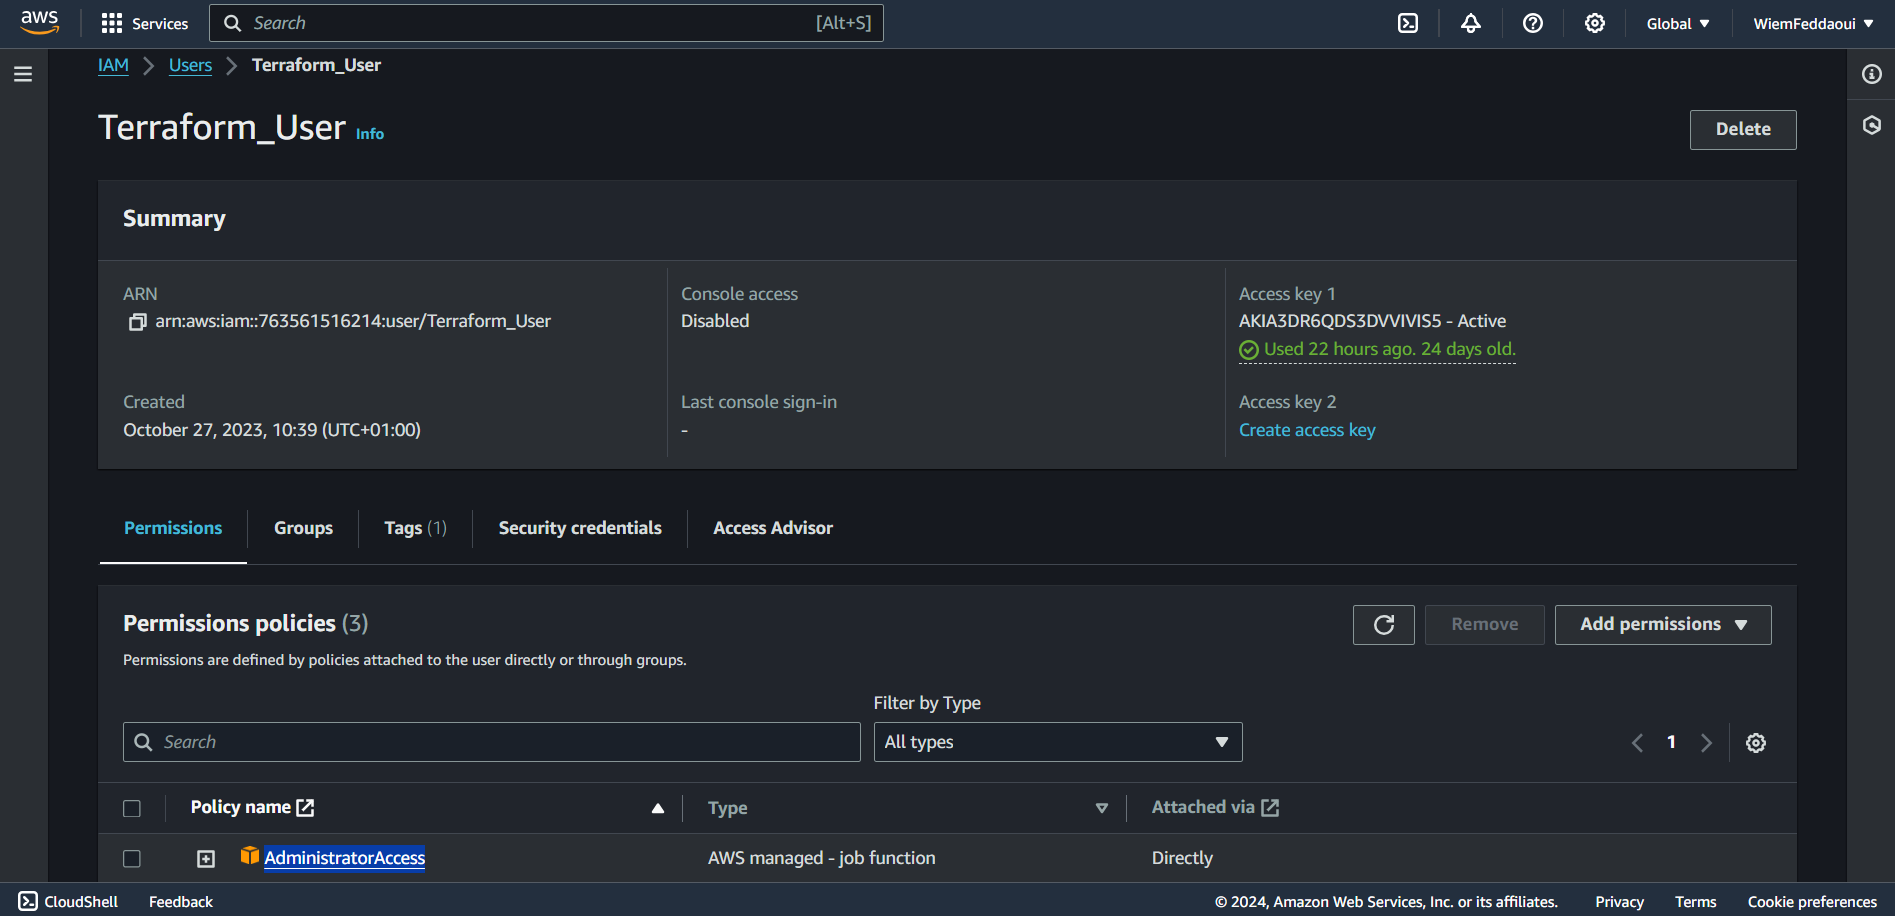
\includegraphics[width=17cm, height=10cm]{img/terraform-user.PNG}}
        \caption{Création d'un utilisateur IAM.}
        \label{fig:terraform_user}
\end{figure}
Cet utilisateur peut avoir des autorisations spécifiques pour contrôler son accès aux ressources AWS, ce qui garantit la sécurité et la gestion des accès aux données et aux services cloud. Dans notre projet, nous attribuons l'accès admin à notre utilisateur IAM.\\ 

La deuxième étape est la création des ressources cloud via Terraform. Nous présentons le code à implémenter afin de créer nos ressources AWS en se basant sur le langage HashiCorp et les coordonnées d'accès de l'utilisateur IAM créé. Ce code est stocké dans le fichier "main.tf". Une partie de ce programme est illustré dans la figure \ref{fig:terraform_main}.
\begin{figure}[H]
        \centering
        \frame{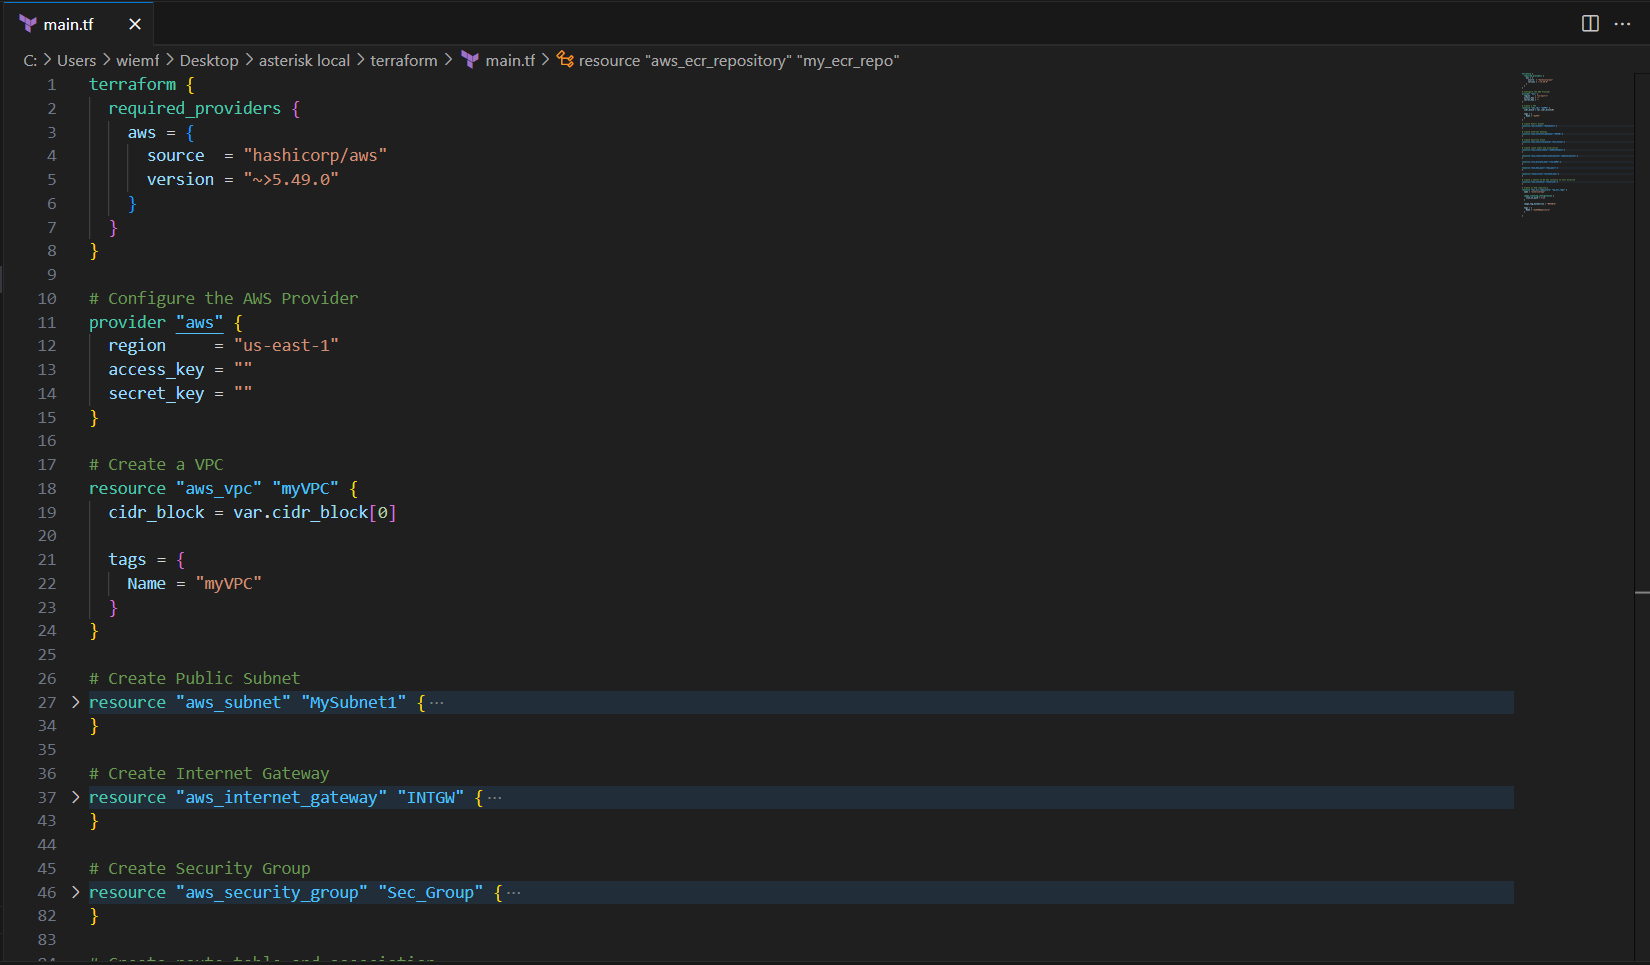
\includegraphics[width=17cm, height=16cm]{img/mainTF.PNG}}
        \caption{Code de création des ressources AWS via Terraform.}
        \label{fig:terraform_main}
\end{figure}
\vspace{2cm}
Nous détaillons alors les ressources à créer :
\begin{itemize}
    \item \textbf{Création d'un VPC:} ce dernier permet de déployer des ressources dans un environnement virtuel isolé, offrant un contrôle total sur leur réseau. Cela inclut la spécification du bloc CIDR définissant l'adresse de ce VPC et l'ajout de tags pour l'identifier.
    \item \textbf{Création d'un Public Subnet:} cette partie décrit la création d'un subnet public dans le VPC précédemment créé. Cette ressource fournit une route vers Internet. Cela signifie que les instances qui se trouvent dans ce subnet peuvent être accessibles depuis Internet.
    \item \textbf{Création d'un Internet Getway:} ici, une passerelle Internet est créée et attachée au VPC. Cette passerelle permet aux ressources du VPC d'accéder à Internet et de recevoir des connexions entrantes depuis le réseau public.
    \item \textbf{Création d'un groupe de sécurité :} cette création définit les règles d'entrée et de sortie du trafic sur des ports spécifiés.
    \item \textbf{Création d'une table de routage et association :} cette partie configure une table de routage pour le VPC, en définissant une route vers l'Internet Getway pour tout le trafic (0.0.0.0/0). Ensuite, la table de routage est associée au subnet public créé précédemment.
    \item \textbf{Génération d'une clé privée :} cette section génère une clé privée RSA de 4096 bits à utiliser pour l'authentification SSH avec l'instance EC2.
    \item \textbf{Création d'une clé public :} une clé publique est créée et elle sera utilisée pour accéder à l'instance EC2.
    \item \textbf{Sauvegarde de la clé privée :} ce bloc de code sauvegarde la clé privée dans un fichier en local. Ce fichier permet l'accès SSH à l'instance EC2.
    \item \textbf{Création d'un dépôt ECR:} ce dépôt créé dans le registre des conteneurs ECR est dédié pour stocker nos images Docker.
    \item \textbf{Création d'une instance EC2 :} cette ressource crée une instance EC2 utilisant l'AMI (Amazon Machine Image) ubuntu 22.04, le type d'instance et la paire de clés générée.\\ L'instance est déployée dans le subnet public, avec une adresse IP publique associée, et elle utilise un script bash d'initialisation pour configurer Docker et Git comme le montre la figure \ref{fig:bash}.
    \begin{figure}[H]
        \centering
        \frame{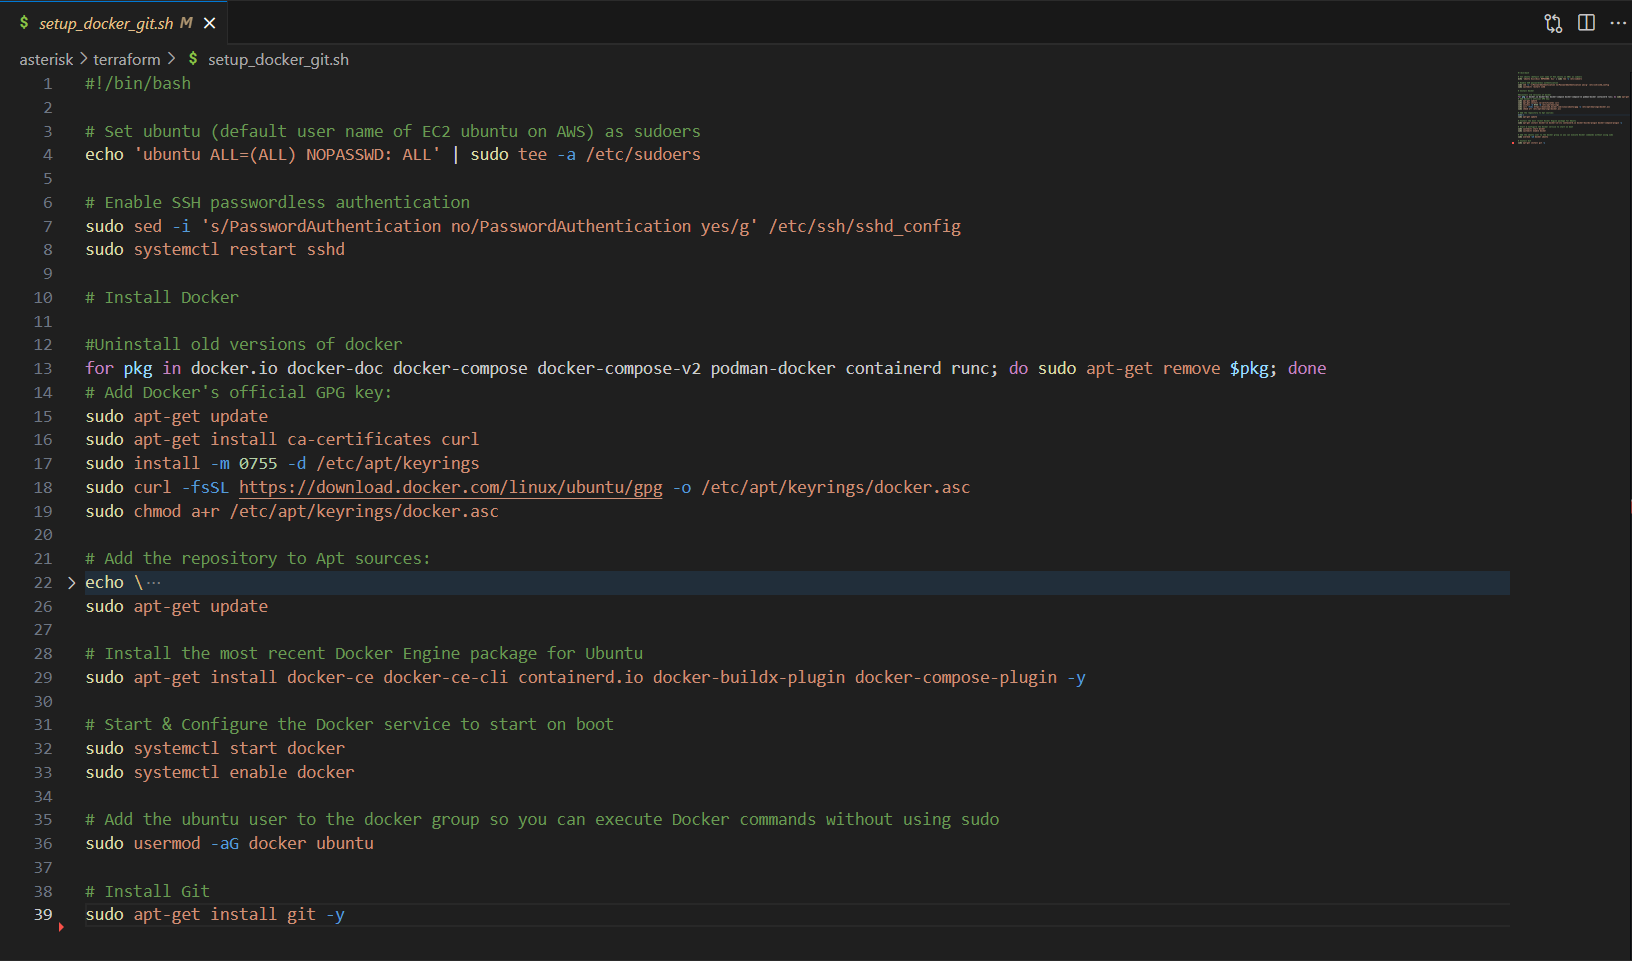
\includegraphics[width=17cm, height=12cm]{img/bash.PNG}}
        \caption{Script bash d'initialisation pour configurer Docker et Git.}
        \label{fig:bash}
    \end{figure}
\end{itemize}

Les variables utilisées dans le fichier "main.tf" sont déclarées dans un fichier "variables.tf", comme le montre la figure \ref{fig:var}.
    \begin{figure}[H]
        \centering
        \frame{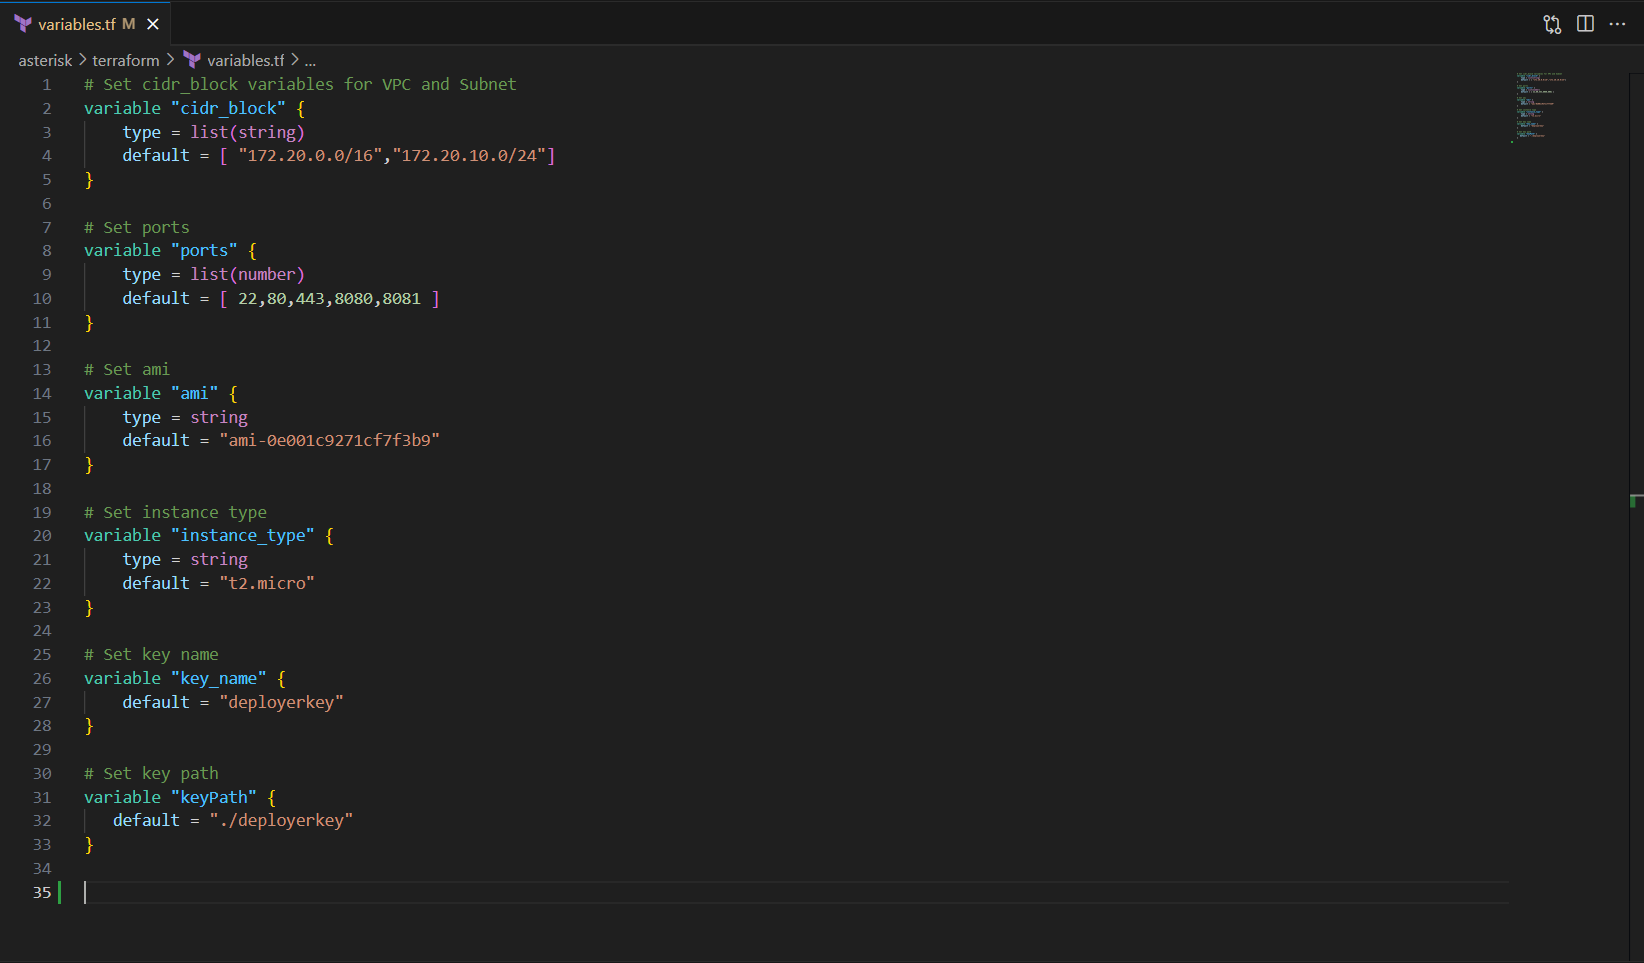
\includegraphics[width=17cm, height=8cm]{img/varTF.PNG}}
        \caption{Code de création des variables Terraform.}
        \label{fig:var}
    \end{figure}

Pour appliquer le code Terraform, nous devons exécuter les trois commandes suivantes :
\begin{itemize}
\item \textbf{Terraform init} pour initialiser le répertoire de travail contenant les fichiers de configuration de Terraform.

\item \textbf{Terraform plan} pour vérifier les modifications qui seront apportées avant de les appliquer.

\item \textbf{Terraform apply} pour appliquer les modifications planifiées.

\end{itemize}

La figure \ref{fig:succes} indique le succès de création de notre infrastructure sur le cloud.
   \begin{figure}[H]
        \centering
        \frame{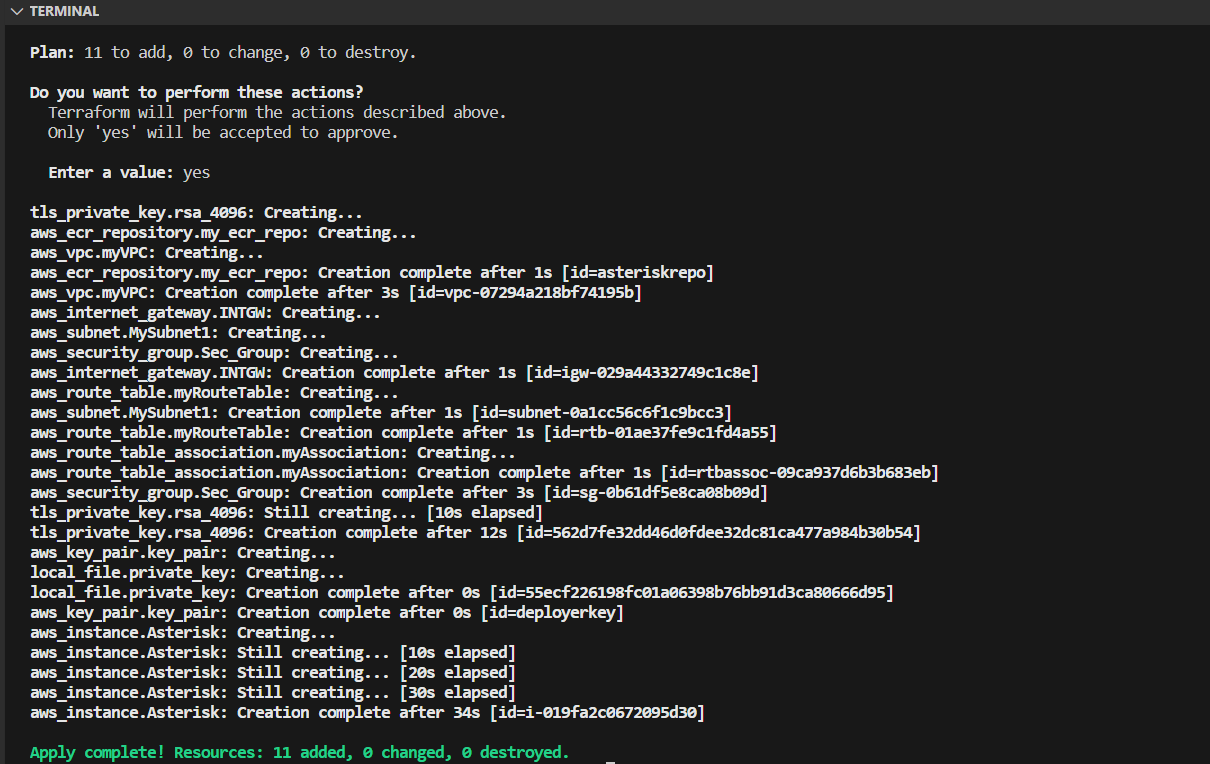
\includegraphics[width=17cm, height=12cm]{img/terminal.PNG}}
        \caption{Succès d'approvisionnement de l'infrastructure.}
        \label{fig:succes}
    \end{figure}

\section{Configuration de serveur Asterisk}
Avant de créer une image Docker pour notre serveur Asterisk, plusieurs fichiers vont être créés et stockées dans /etc/asterisk/. Nous présentons alors ces fichiers et leurs configurations.
\begin{itemize}
    \item \textbf{asterisk.conf:}  ce fichier définit les variables nécessaires à l’utilisation d’Asterisk. Il sert à guider
Asterisk où il doit chercher certains fichiers et les programmes exécutables.\\ La figure \ref{fig:ast} présente le code du fichier.
   \begin{figure}[H]
        \centering
        \frame{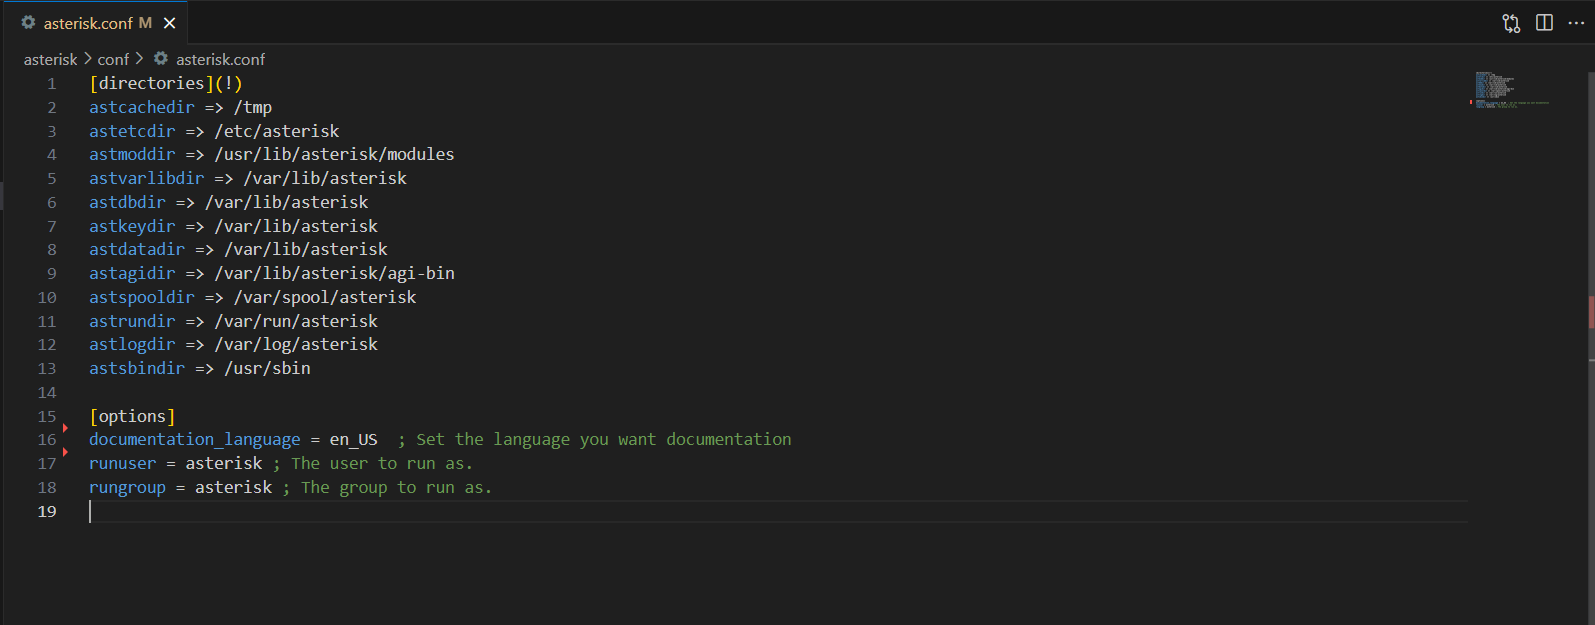
\includegraphics[width=17cm, height=12cm]{img/ast-conf.PNG}}
        \caption{Configuration du fichier "asterisk.conf".}
        \label{fig:ast}
    \end{figure}
    \item \textbf{extconfig.conf:} ce fichier est utilisé pour configurer les sources externes du serveur Asterisk. Il permet d’utiliser des bases de données externes pour stocker des configurations spécifiques. La figure \ref{fig:ext} présente le code du fichier.
   \begin{figure}[H]
        \centering
        \frame{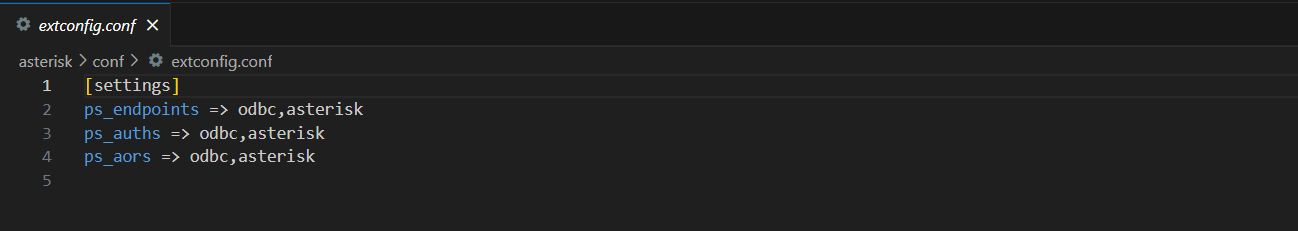
\includegraphics[width=17cm, height=5cm]{img/extconfig.PNG}}
        \caption{Configuration du fichier "extconfig.conf".}
        \label{fig:ext}
    \end{figure}
    \item \textbf{extensions.conf:} ce fichier est utilisé pour définir le plan de numérotation d’Asterisk. Il décrit comment les appels sont traités, dirigés et quelles actions sont effectuées pour chaque numéro composé. La figure \ref{fig:exts} présente le code du fichier.
   \begin{figure}[H]
        \centering
        \frame{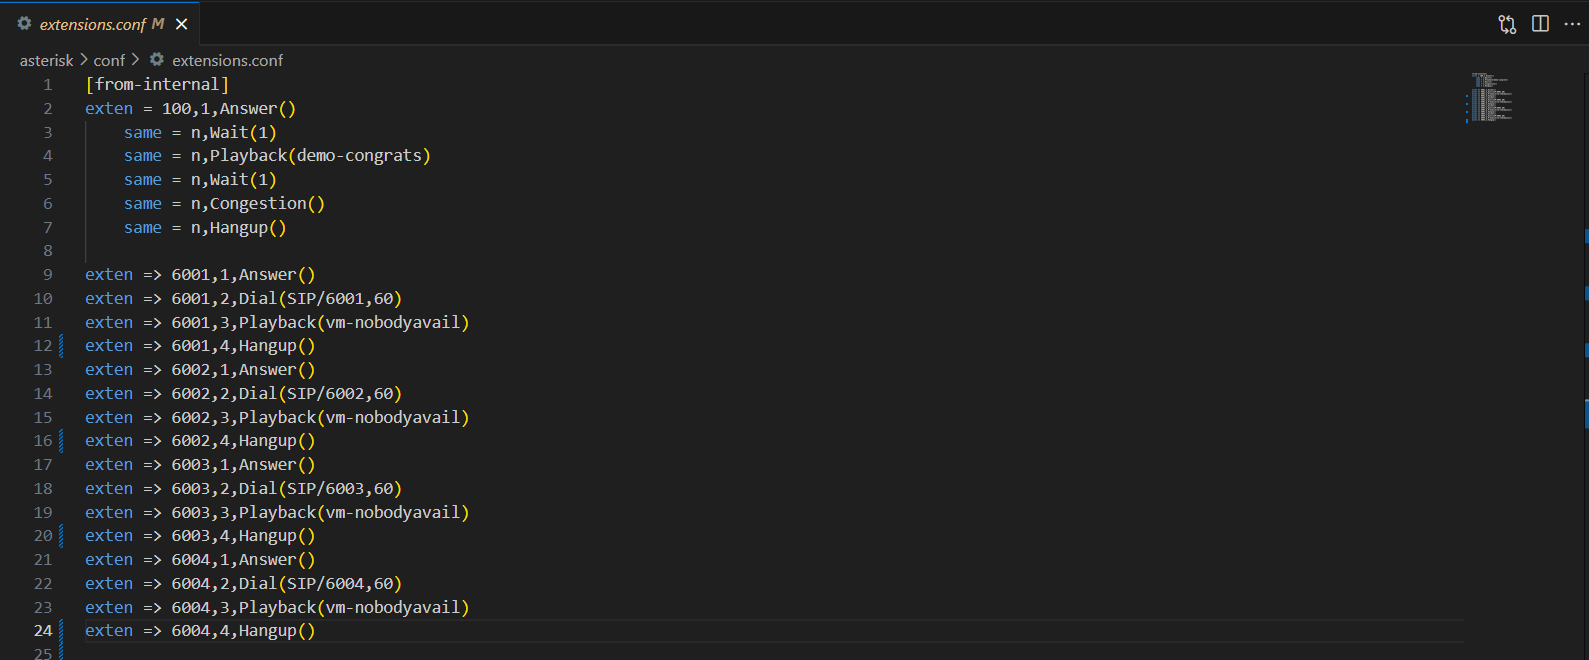
\includegraphics[width=17cm, height=11cm]{img/extensions.PNG}}
        \caption{Configuration du fichier "extensions.conf".}
        \label{fig:exts}
    \end{figure}
    \item \textbf{modules.conf:} ce fichier contrôle quels modules sont chargés ou non au démarrage d’Asterisk. Il permet de gérer les fonctionnalités disponibles dans Asterisk en activant ou désactivant les modules. La figure \ref{fig:mod} présente le code du fichier.
   \begin{figure}[H]
        \centering
        \frame{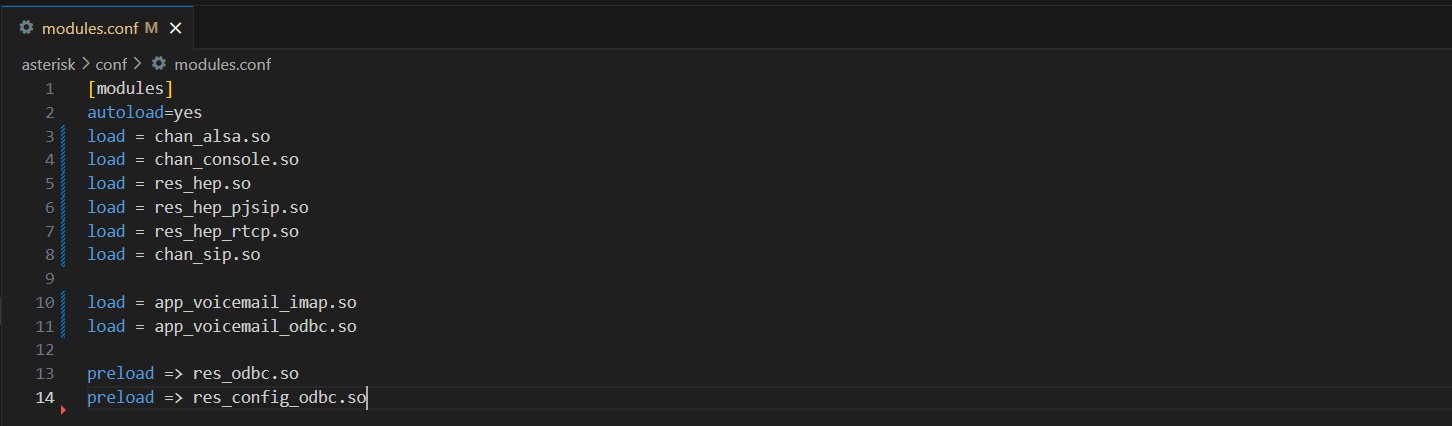
\includegraphics[width=17cm, height=7cm]{img/modules.PNG}}
        \caption{Configuration du fichier "modules.conf".}
        \label{fig:mod}
    \end{figure}
    \item \textbf{pjsip.conf:} ce fichier configure le module PJSIP, utilisé pour la gestion des protocoles SIP dans Asterisk. Il remplace l’ancien sip.conf pour une gestion plus flexible et plus performante des connexions SIP. La figure \ref{fig:pjsip} présente le code du fichier.
   \begin{figure}[H]
        \centering
        \frame{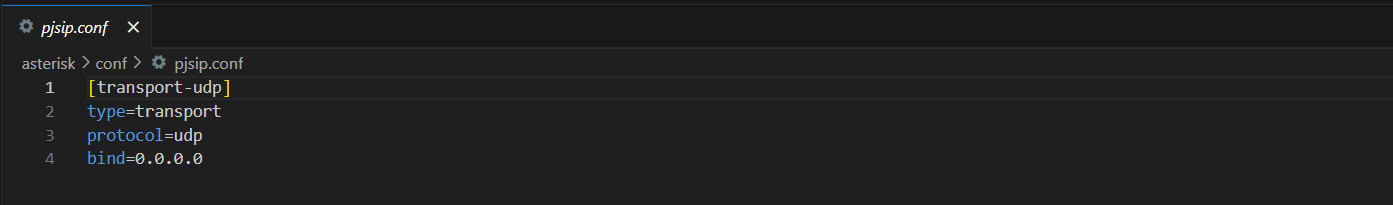
\includegraphics[width=17cm, height=5cm]{img/pjsip.PNG}}
        \caption{Configuration du fichier "pjsip.conf".}
        \label{fig:pjsip}
    \end{figure}
    \item \textbf{res_odbc.conf:} ce fichier configure les connexions ODBC pour Asterisk, permettant à celui-ci de se connecter à des bases de données relationnelles pour des tâches telles que la gestion des CDR (Call Detail Records) et les répertoires de numérotation. La figure \ref{fig:odbc} présente le code du fichier.
   \begin{figure}[H]
        \centering
        \frame{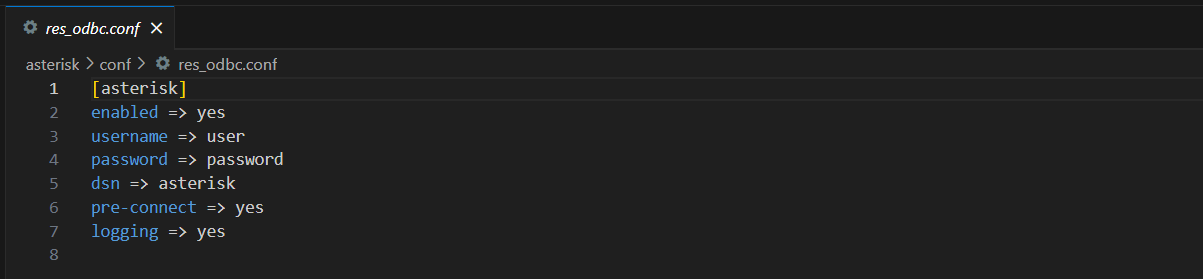
\includegraphics[width=17cm, height=6cm]{img/res_odbc.PNG}}
        \caption{Configuration du fichier "res_odbc.conf".}
        \label{fig:odbc}
    \end{figure}
    \item \textbf{sorcery.conf:} ce fichier configure le système Sorcery d’Asterisk, qui est utilisé pour la gestion des données de configuration en utilisant différents backends de stockage. Il permet de spécifier comment et où les différentes catégories de données de configuration sont stockées et récupérées. La figure \ref{fig:sorcery} présente le code du fichier.
   \begin{figure}[H]
        \centering
        \frame{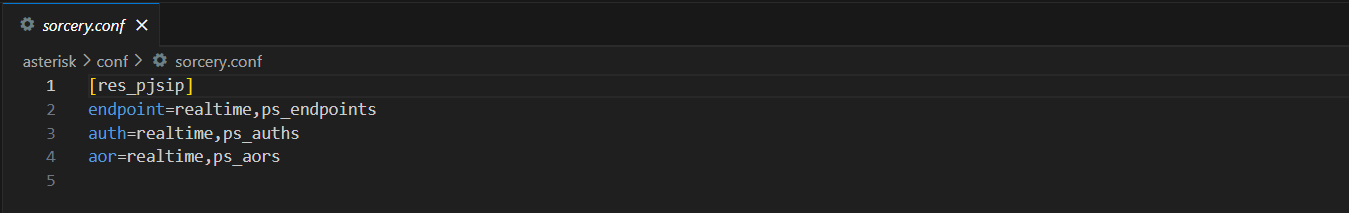
\includegraphics[width=17cm, height=4cm]{img/sorcery.PNG}}
        \caption{Configuration du fichier "sorcery.conf".}
        \label{fig:sorcery}
    \end{figure}
\end{itemize}
Ces fichiers de configuration nous permettent de personnaliser et de contrôler le fonctionnement d’Asterisk. Chacun joue un rôle spécifique dans la gestion des appels, des modules, des protocoles et des connexions aux bases de données, offrant une flexibilité et une extensibilité importante à ce serveur de communication.

\section{Configuration de la base de données MySQL}
Un dump est une sauvegarde de la base de données, souvent utilisée pour restaurer la base de données ou la transférer vers un autre serveur. Dans cette partie, nous créons ce fichier pour définir la structure et les données de certaines tables de la base de données Asterisk. 
\begin{itemize}
    \item La table \texttt{ps\_aors} est définie pour stocker les informations sur les AORs (Address of Records), qui sont des points de contact pour les utilisateurs SIP.
    \item La table \texttt{ps\_auths} contient des informations d'authentification pour les utilisateurs SIP.
    \item La table \texttt{ps\_endpoints} définit les points de terminaison (endpoints) SIP, qui sont les appareils ou logiciels utilisés pour les appels.
\end{itemize}
La figure \ref{fig:dumb} illustre une partie du code de ce fichier.
   \begin{figure}[H]
        \centering
        \frame{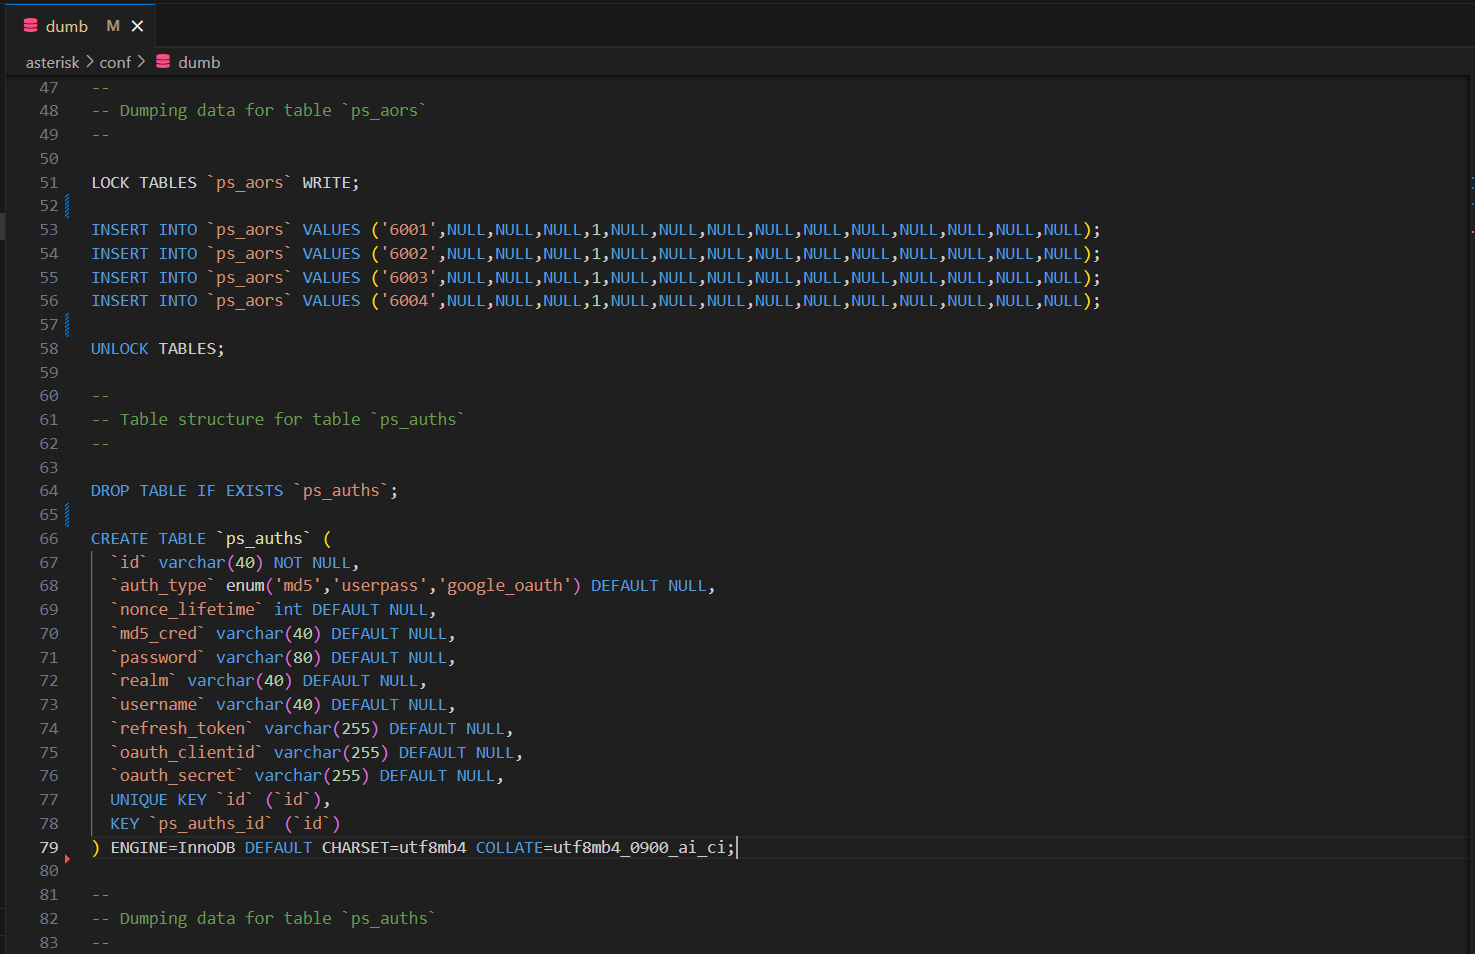
\includegraphics[width=17cm, height=13cm]{img/dumb.PNG}}
        \caption{Configuration du fichier "dumb.sql".}
        \label{fig:dumb}
    \end{figure}

\section{Construction d'une image Docker pour Asterisk} 
La construction d'une image Docker pour le serveur Asterisk implique la création d'un fichier Dockerfile spécifique pour Asterisk, comme illustré dans la figure \ref{fig:dc1}. Ce fichier contient toutes les dépendances, les configurations de port et l'environnement nécessaires pour construire le serveur. L'objectif est de générer une image isolée du reste du code. Cette étape sera intégrée à la première phase de la réalisation du pipeline CI/CD.
\begin{figure}[H]
        \centering
        \frame{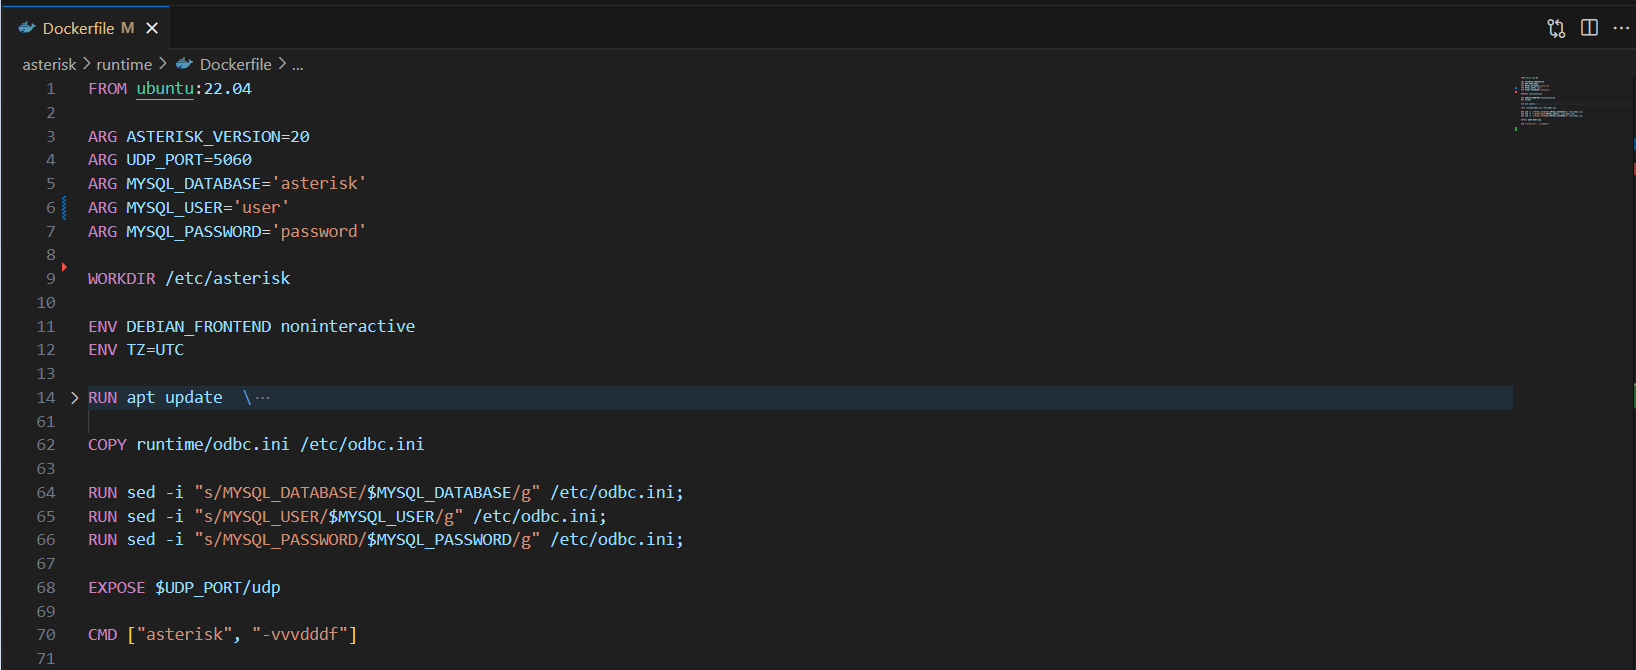
\includegraphics[width=17cm, height=11cm]{img/dockerfile_asterisk.PNG}}
        \caption{Dockerfile du serveur Asterisk.}
        \label{fig:dc1}
        \end{figure}
        
\section{Conteneurisation de l'image Docker Asterisk} 
Cette partie est consacrée à la conteneurisation qui vise à rendre une image Docker exécutable sur n'importe quelle infrastructure.

Pour exécuter l'images Docker créée précédemment, nous utilisons un fichier «docker-compose.yml» présenté dans la figure \ref{fig:dc3}. Ce fichier permet de lancer l'image du serveur Asterisk en parallèle avec l'image de base de données MySQL fournie par Docker. Nous obtenons ainsi deux conteneurs qui sont placés dans le même réseau et peuvent communique ensemble.
\begin{figure}[H]
        \centering
        \frame{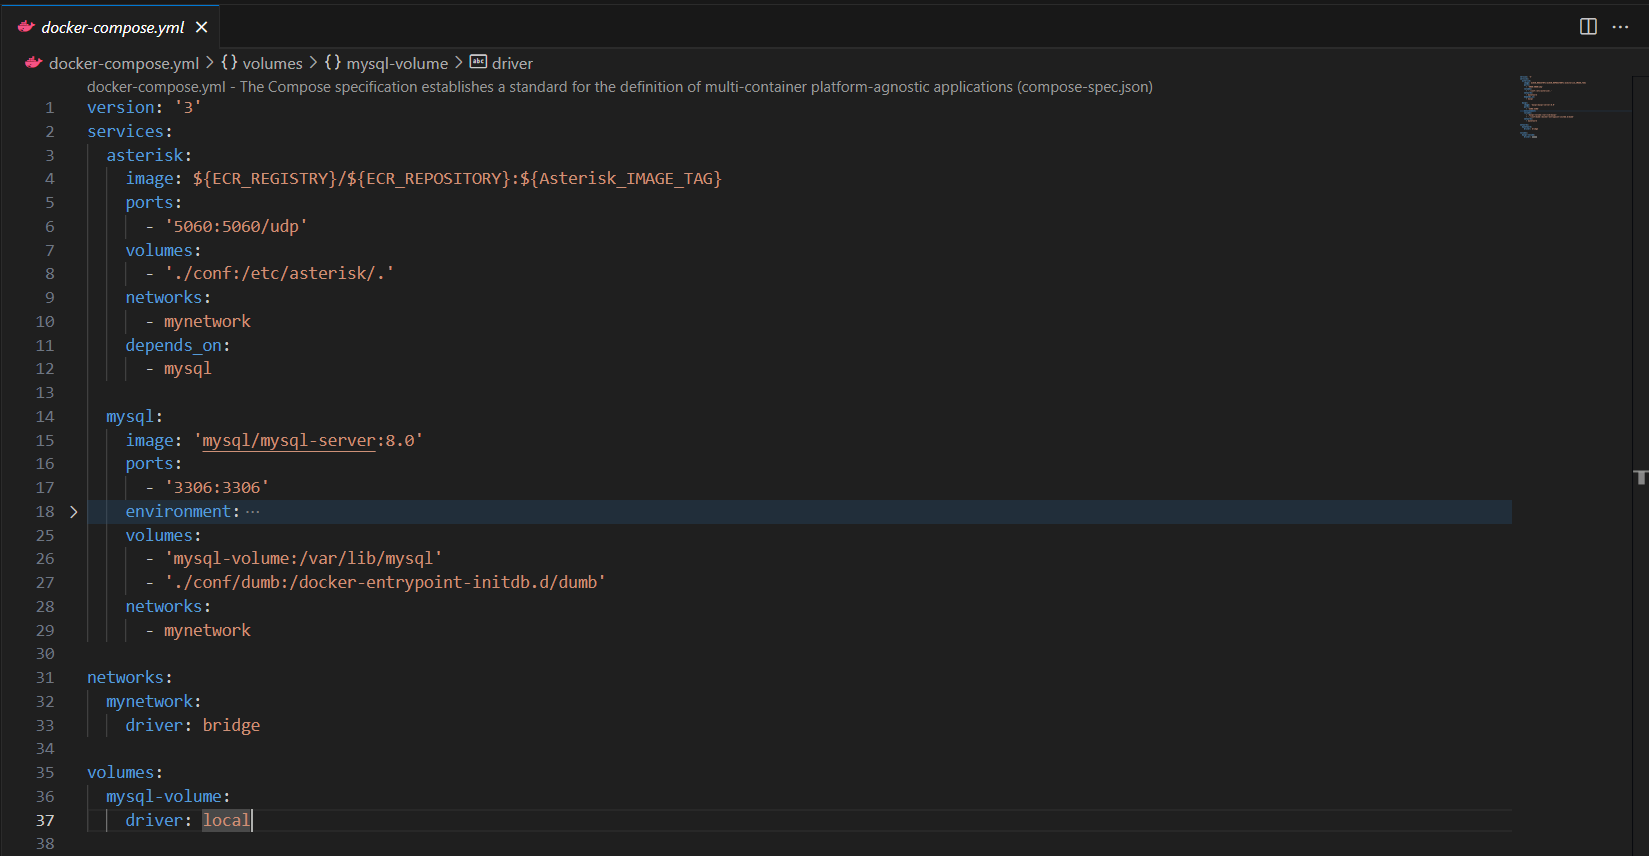
\includegraphics[width=17cm, height=14cm]{img/docker-compose.PNG}}
        \caption{Docker Compose du système Asterisk.}
        \label{fig:dc3}
        \end{figure}

\section{Mise en place d'un pipeline CI/CD}

Après avoir préparé les phases nécessaires pour le pipeline CI/CD d'Asterisk, nous créons le code de ce pipeline et le testons à travers GitHub Actions. Dès qu’un changement est détecté au niveau du code, le pipeline se déclenche automatiquement.
Ce dernier illustré par la figure \ref{fig:cicd}, nommé "Build and Deploy", gère le processus de construction et de déploiement de notre solution utilisant Docker Compose sur une instance EC2.

La section "build" construit et pousse l'image Docker d'Asterisk vers Amazon ECR, tandis que la section "deploy" déploie cette image sur l'instance EC2 spécifiée. Elle supprime également l'ancienne configuration Docker Compose de l'instance, copie les nouveaux fichiers de configuration et les fichiers de configuration d'Asterisk, puis utilise Docker Compose pour démarrer les conteneurs.

En outre, le script de déploiement mentionne la création d'un fichier ".env", qui semble être utilisé pour définir des variables d'environnement nécessaires au déploiement, telles que le registre ECR, le référentiel ECR et le tag de l'image Asterisk. Cependant, il y a une mention d'un fichier "dumb" dans le commentaire final.
\begin{itemize}
    \item Build and Push Asterisk image to ECR : construction et envoi de l’image Docker vers le service ECR d’AWS pour la stocker.
    \item Deploy : l’importation de l’image Docker du serveur Asterisk stockée dans le service ECR et le lancement de Docker Compose sur l’instance EC2 avec un serveur base de données MySQL.
\end{itemize}

\begin{figure}[H]
        \centering
        \frame{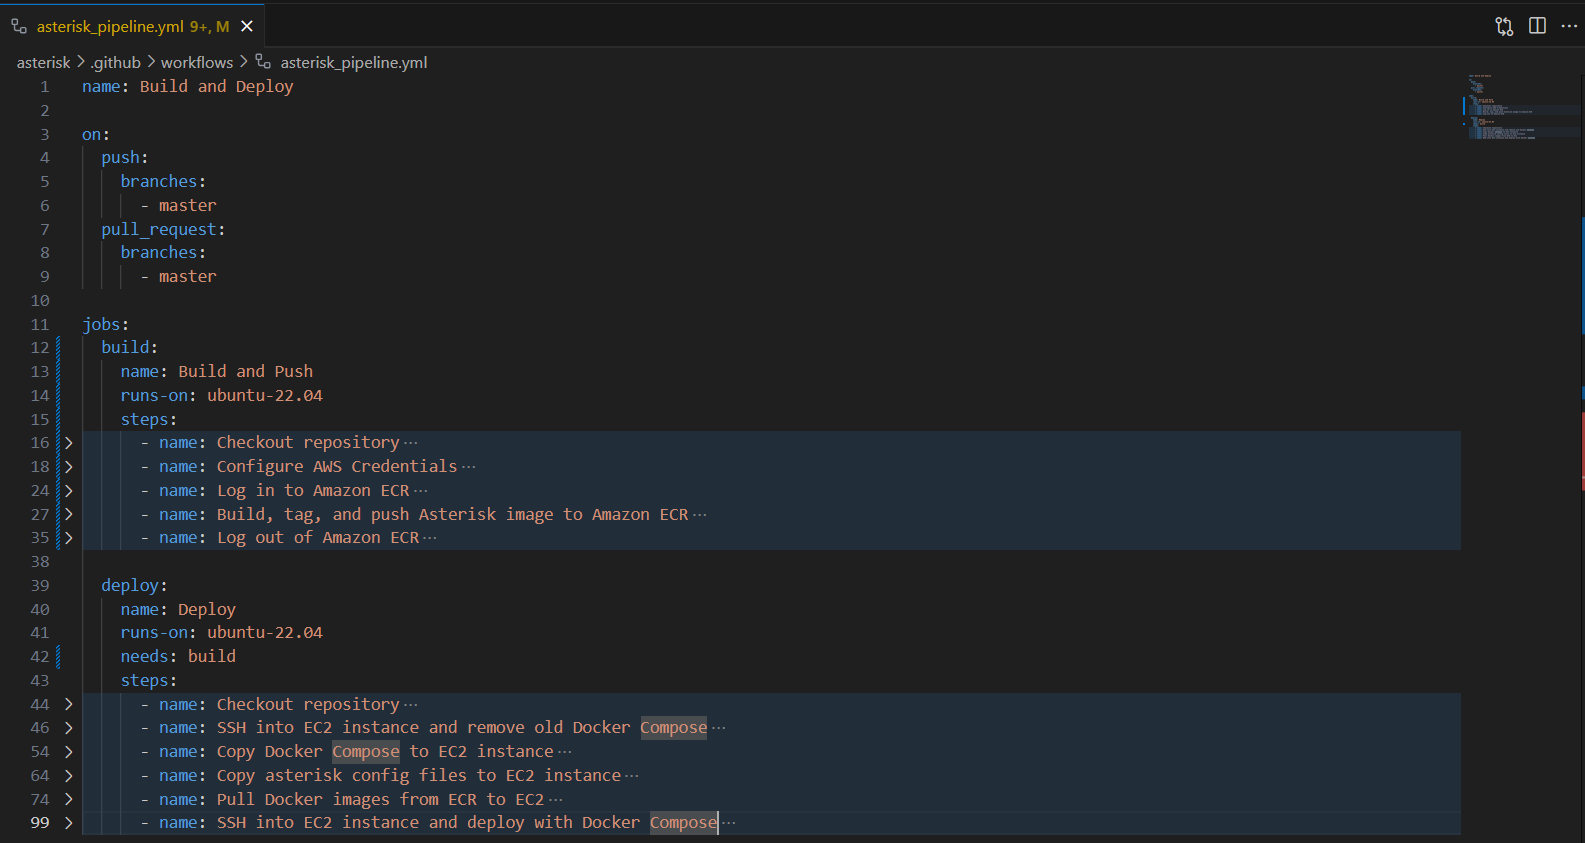
\includegraphics[width=17cm, height=14cm]{img/pipe.PNG}}
        \caption{Pipeline CI/CD du système Asterisk.}
        \label{fig:cicd}
        \end{figure}

La figure \ref{fig:s} présente graphiquement les étapes du pipeline CI/CD du système Asterisk et indique le succès de chaque phase.
\begin{figure}[H]
        \centering
        \frame{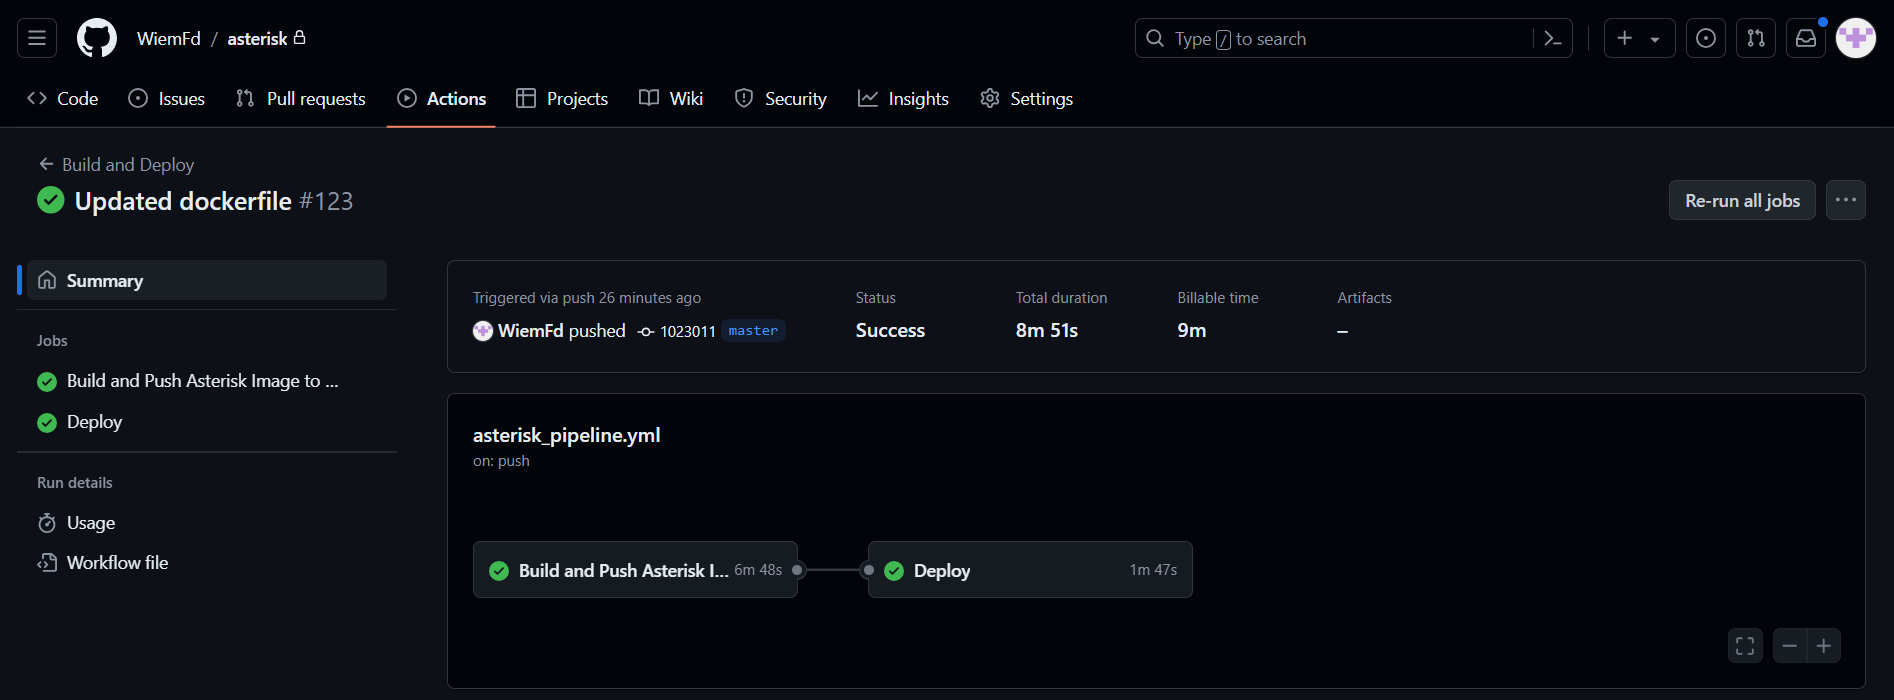
\includegraphics[width=17cm, height=9cm]{img/pipeline_s.PNG}}
        \caption{Représentation graphique de pipeline CI/CD.}
        \label{fig:s}
\end{figure}
Lors de la création du code de pipeline CI/CD, des données sensibles comme les clés d'accès à notre compte AWS, ne doivent pas être affichées en texte clair. Grâce au GitHub Secrets, nous pouvons stockées nos variables de manière cryptée et sécurisé comme le montre la figure \ref{fig:secrets}.
\begin{figure}[H]
        \centering
        \frame{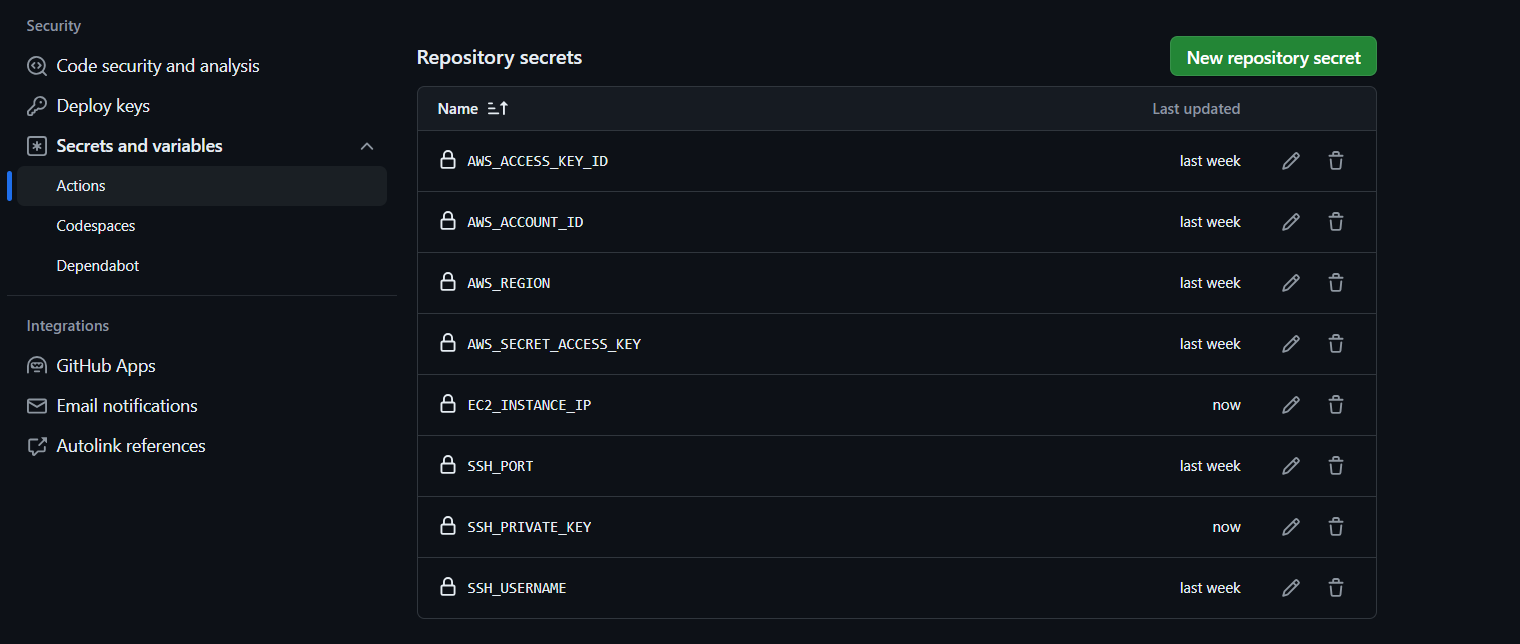
\includegraphics[width=17cm, height=9cm]{img/secrets.PNG}}
        \caption{Stockage des données sensibles sur Github.}
        \label{fig:secrets}
\end{figure}

\section{Test et validation de l'accès au seveur Asterisk}
Dès que le pipeline se termine, les conteneurs Docker seront déployés sur notre instance ubuntu EC2. Pour assurer que ces conteneurs sont créés correctement et en cours d'exécution. Nous devons appliquer la commande "docker ps" présentée dans la figure \ref{fig:ps}.
\begin{figure}[H]
        \centering
        \frame{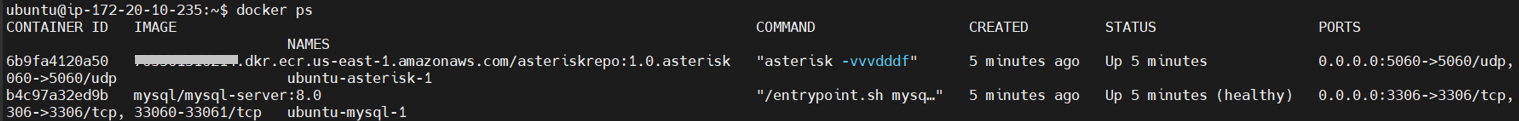
\includegraphics[width=17cm, height=3cm]{img/docker_ps.PNG}}
        \caption{Succès de création des conteneurs Docker.}
        \label{fig:ps}
\end{figure}

Tout d'abord, nous devons établir une connexion SSH avec l'instance AWS via la clé privée copiée en locale lors du processus de l'approvisionnement. Maintenant, nous pouvons accéder à ce conteneur et vérifier le bon fonctionnement de notre service Asterisk en suivant les commandes illustrées dans la figure \ref{fig:ok-asterisk}. 
\begin{figure}[H]
        \centering
        \frame{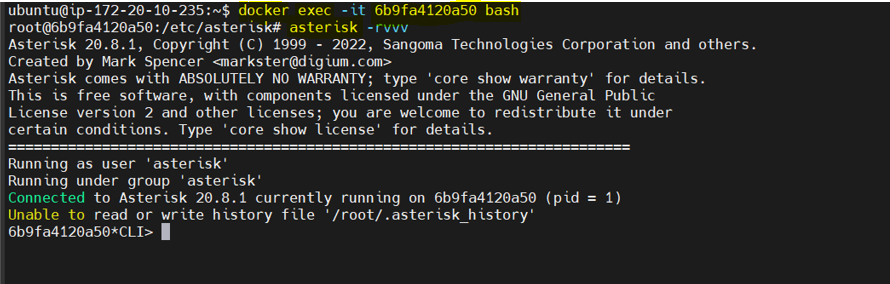
\includegraphics[width=17cm, height=6cm]{img/asterisk-s.PNG}}
        \caption{Succès d'accès au service Asterisk.}
        \label{fig:ok-asterisk}
\end{figure}
Afin de tester un appel audio via Asterisk, nous utilisons l'application client Linphone basée sur le protocole d'initiation SIP.
Cette application possède une version Desktop et une version mobile. Pour se connecter, nous devons utilisés l'adresse publique de notre instance comme domaine SIP, un nom d'utilisateur crée déjà dans notre base de données MySQL ainsi que son mot de passe. Il est important aussi de vérifier si Linphone utilise le port d'accès au serveur Asterisk 5060. Dès que la connexion s'établie, nous tappons 100 pour écouter le message vocale de succès de configuration "demo-congrats".
La figure \ref{fig:ok-linphone} illustre cet appel.
\begin{figure}[H]
        \centering
        \frame{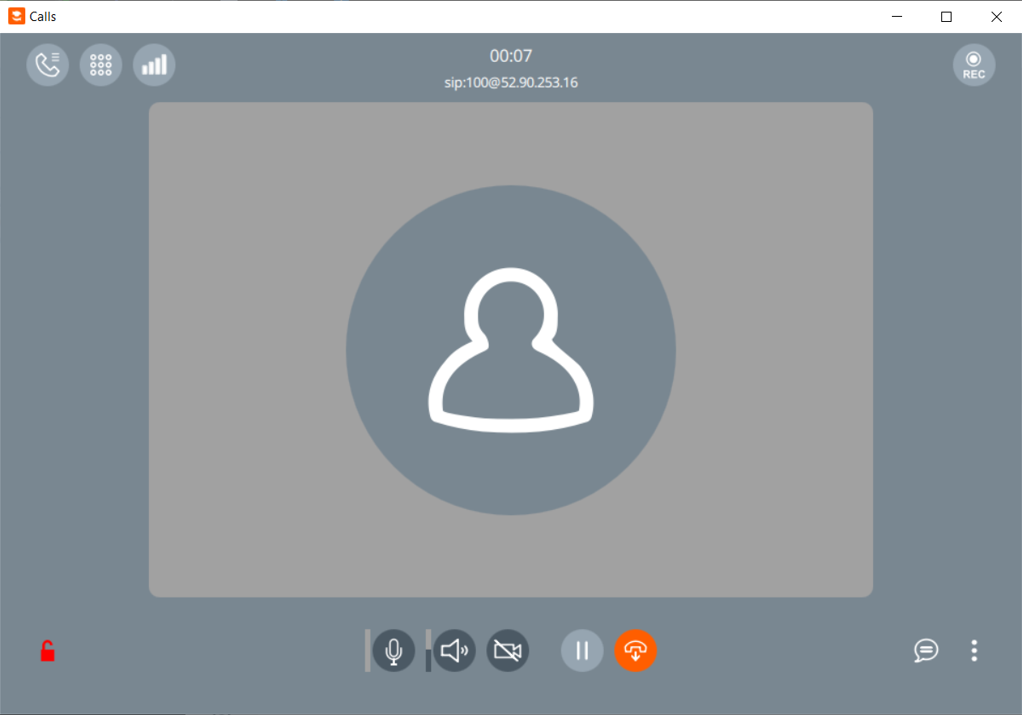
\includegraphics[width=17cm, height=7.25cm]{img/linphone_call.PNG}}
        \caption{Accès au serveur Asterisk à partir de Linphone.}
        \label{fig:ok-linphone}
\end{figure}

\section{Personnalisation de l'application Linphone}
L'application Desktop client Linphone SIP est open-source et développée avec QML/QT5 et C++. Pour commencer à personnaliser cette application, il faut préparer l'environnement de développement et installer les dépendances nécessaires. Le nom est transformé au Bridge et le style de l'application est modifié, comme présenté dans la figure \ref{fig:linphone}.
\begin{figure}[H]
        \centering
      \frame{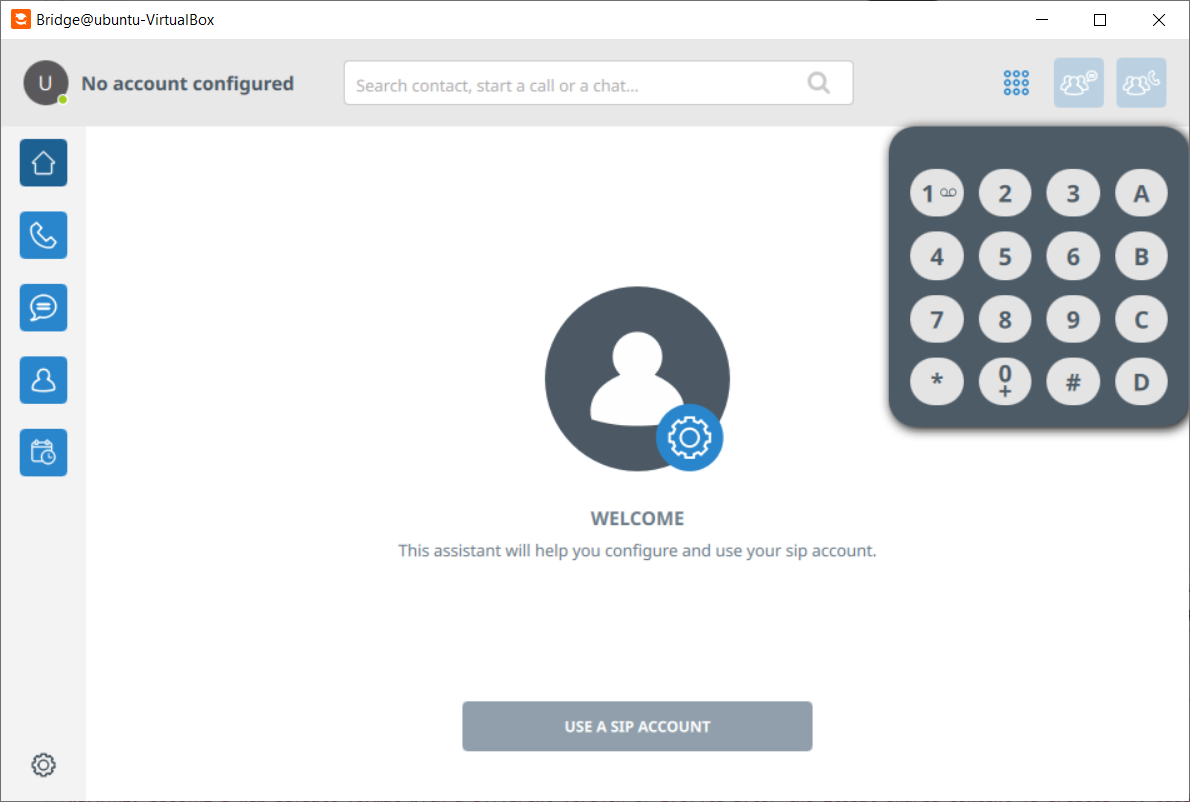
\includegraphics[width=17cm, height=10cm]{img/linphone.PNG}}
        \caption{Application Bridge.}
        \label{fig:linphone}
\end{figure}

\section*{Conclusion}
Ce chapitre nous a permis de présenter, dans un premier temps, la mise en place de la solution en couvrant l'approvisionnement de l'IaC, la création de l'image Docker pour Asterisk, ainsi que la conteneurisation du serveur et la mise en place des phases du pipeline CI/CD. Enfin, nous avons mis en évidence le test et la validation de la connexion au service Asterisk, ainsi que la personnalisation de l'application client Linphone.








        \clearpage
        
        \chapter*{Conclusion générale}
\addcontentsline{toc}{chapter}{Conclusion générale}
\markboth{Conclusion générale}{}
%\paragraph{}
L'intégration de l'IaC, l'adoption de l'approche DevOps et l'automatisation de l'intégration et du déploiement continus sur AWS Cloud sont des tendances significatives qui ont profondément influencé notre projet. Lorsqu'elles sont combinées, ces pratiques créent une agilité remarquable et une efficacité accrue.
\\

Dans ce contexte, notre projet a atteint son objectif en accélérant le déploiement et en assurant la satisfaction du client. Nous avons établi une infrastructure cloud automatisée pour héberger notre serveur Asterisk et sa base de données MySQL. De plus, nous avons mis en place un pipeline d'intégration continue et de déploiement continu pour Asterisk, en utilisant l'application client Linphone pour tester la fonctionnalité d'appel.
\\

Ce stage de fin d'études m'a permis de m'immerger dans la vie professionnelle, en appliquant les connaissances techniques acquises pendant mes années d'études à l'Institut Supérieur d'Informatique. Mon expérience chez Luceor Labs, bien que brève, m'a permis de découvrir de nouveaux concepts liés à l'infrastructure en tant que code, à l'approche DevOps et au cloud public, tout en interagissant avec des professionnels du secteur et en recevant des conseils précieux qui ont renforcé mes compétences en communication et en travail d'équipe.
\\

Pour améliorer encore notre projet, nous pourrions envisager d'ajouter une solution Kubernetes Replica-set pour réduire la charge sur la base de données. De plus, une solution automatique de sauvegarde des backups pourrait être mise en place. Il serait également nécessaire d'étendre les tests sur notre serveur Asterisk à d'autres fonctionnalités critiques telles que Push-to-Talk et la messagerie instantanée. Enfin, il reste à aborder la phase de transition vers l'environnement de production du serveur Asterisk, en mettant l'accent sur la sécurisation des ports, l'utilisation d'un nom de domaine et la préparation à la présentation aux utilisateurs finaux.

        \clearpage
        
        % @author: Stoufa
		% the command `\nocite{*}` is mandatory to avoid the “no \citation commands” error
        % https://tex.stackexchange.com/questions/18045/problem-with-compiling-bibtex-no-citation-commands-error
        %\nocite{*}
        \printbibliography[heading=bibintoc]
        
        




        \clearpage

    \backmatter
        %===== File containing the back cover of the document =====%
%                                                          %
% Copyright (C) ISI - All Rights Reserved                  %
% Proprietary                                              %
% Written by Med Hossam <med.hossam@gmail.com>, April 2016 %
%                                                          %
% @author: HEDHILI Med Houssemeddine                       %
% @linkedin: http://tn.linkedin.com/in/medhossam           %
%==========================================================%

%== It's advised to not modify the content of this file ===%
% To set your information, go to global_config.tex file    %
%==========================================================%

\thispagestyle{backcover}
\newgeometry{bottom=25mm,left=15mm,top=20mm,right=15mm}

\begin{changemargin}{3mm}{0cm}
    \begin{minipage}[c]{0.96\columnwidth}
        
        \selectlanguage{arabic}
        
        {\LARGE\textbf{ملخّص}}
        \vskip1mm
            \begingroup
                \small
                \@arabicAbstract
            \endgroup
        \vskip1mm
        {\textbf{كلمات مفاتيح : } 
            \begingroup
                \@arabicAbstractKeywords
            \endgroup
        }
        
        {\ifthenelse{\boolean{wantToTypeCompanyAddress}}
        {% IF TRUE
            \vskip5mm
        }{\vskip8mm}}
        
        \selectlanguage{french}
        
        {\LARGE\textbf{Résumé}}
        \vskip1mm
            \begingroup
                \large
                \@frenchAbstract
            \endgroup
        \vskip1mm
        {\textbf{Mots clés : }
            \begingroup
                \@frenchAbstractKeywords
            \endgroup
        }
        
        {\ifthenelse{\boolean{wantToTypeCompanyAddress}}
        {% IF TRUE
            \vskip5mm
        }{\vskip8mm}}
        
        \selectlanguage{english}
        {\LARGE\textbf{Abstract}}
        \vskip1mm
            \begingroup
                \large
                \@englishAbstract
            \endgroup
        \vskip1mm
        {\textbf{Keywords : }
            \begingroup
                \@englishAbstractKeywords
            \endgroup
        }
    \end{minipage}
    
\end{changemargin}
    
\end{document}